
%% bare_jrnl_compsoc.tex
%% V1.4b
%% 2015/08/26
%% by Michael Shell
%% See:
%% http://www.michaelshell.org/
%% for current contact information.
%%
%% This is a skeleton file demonstrating the use of IEEEtran.cls
%% (requires IEEEtran.cls version 1.8b or later) with an IEEE
%% Computer Society journal paper.
%%
%% Support sites:
%% http://www.michaelshell.org/tex/ieeetran/
%% http://www.ctan.org/pkg/ieeetran
%% and
%% http://www.ieee.org/

%%*************************************************************************
%% Legal Notice:
%% This code is offered as-is without any warranty either expressed or
%% implied; without even the implied warranty of MERCHANTABILITY or
%% FITNESS FOR A PARTICULAR PURPOSE! 
%% User assumes all risk.
%% In no event shall the IEEE or any contributor to this code be liable for
%% any damages or losses, including, but not limited to, incidental,
%% consequential, or any other damages, resulting from the use or misuse
%% of any information contained here.
%%
%% All comments are the opinions of their respective authors and are not
%% necessarily endorsed by the IEEE.
%%
%% This work is distributed under the LaTeX Project Public License (LPPL)
%% ( http://www.latex-project.org/ ) version 1.3, and may be freely used,
%% distributed and modified. A copy of the LPPL, version 1.3, is included
%% in the base LaTeX documentation of all distributions of LaTeX released
%% 2003/12/01 or later.
%% Retain all contribution notices and credits.
%% ** Modified files should be clearly indicated as such, including  **
%% ** renaming them and changing author support contact information. **
%%*************************************************************************


% *** Authors should verify (and, if needed, correct) their LaTeX system  ***
% *** with the testflow diagnostic prior to trusting their LaTeX platform ***
% *** with production work. The IEEE's font choices and paper sizes can   ***
% *** trigger bugs that do not appear when using other class files.       ***                          ***
% The testflow support page is at:
% http://www.michaelshell.org/tex/testflow/


\documentclass[10pt,journal,compsoc]{IEEEtran}
%
% If IEEEtran.cls has not been installed into the LaTeX system files,
% manually specify the path to it like:
% \documentclass[10pt,journal,compsoc]{../sty/IEEEtran}





% Some very useful LaTeX packages include:
% (uncomment the ones you want to load)


% *** MISC UTILITY PACKAGES ***
%
%\usepackage{ifpdf}
% Heiko Oberdiek's ifpdf.sty is very useful if you need conditional
% compilation based on whether the output is pdf or dvi.
% usage:
% \ifpdf
%   % pdf code
% \else
%   % dvi code
% \fi
% The latest version of ifpdf.sty can be obtained from:
% http://www.ctan.org/pkg/ifpdf
% Also, note that IEEEtran.cls V1.7 and later provides a builtin
% \ifCLASSINFOpdf conditional that works the same way.
% When switching from latex to pdflatex and vice-versa, the compiler may
% have to be run twice to clear warning/error messages.






% *** CITATION PACKAGES ***
%
\ifCLASSOPTIONcompsoc
  % IEEE Computer Society needs nocompress option
  % requires cite.sty v4.0 or later (November 2003)
  \usepackage[nocompress]{cite}
\else
  % normal IEEE
  \usepackage{cite}
\fi
% cite.sty was written by Donald Arseneau
% V1.6 and later of IEEEtran pre-defines the format of the cite.sty package
% \cite{} output to follow that of the IEEE. Loading the cite package will
% result in citation numbers being automatically sorted and properly
% "compressed/ranged". e.g., [1], [9], [2], [7], [5], [6] without using
% cite.sty will become [1], [2], [5]--[7], [9] using cite.sty. cite.sty's
% \cite will automatically add leading space, if needed. Use cite.sty's
% noadjust option (cite.sty V3.8 and later) if you want to turn this off
% such as if a citation ever needs to be enclosed in parenthesis.
% cite.sty is already installed on most LaTeX systems. Be sure and use
% version 5.0 (2009-03-20) and later if using hyperref.sty.
% The latest version can be obtained at:
% http://www.ctan.org/pkg/cite
% The documentation is contained in the cite.sty file itself.
%
% Note that some packages require special options to format as the Computer
% Society requires. In particular, Computer Society  papers do not use
% compressed citation ranges as is done in typical IEEE papers
% (e.g., [1]-[4]). Instead, they list every citation separately in order
% (e.g., [1], [2], [3], [4]). To get the latter we need to load the cite
% package with the nocompress option which is supported by cite.sty v4.0
% and later. Note also the use of a CLASSOPTION conditional provided by
% IEEEtran.cls V1.7 and later.





% *** GRAPHICS RELATED PACKAGES ***
%
\ifCLASSINFOpdf
  \usepackage[pdftex]{graphicx}
  % declare the path(s) where your graphic files are
  % \graphicspath{{../pdf/}{../jpeg/}}
  % and their extensions so you won't have to specify these with
  % every instance of \includegraphics
  % \DeclareGraphicsExtensions{.pdf,.jpeg,.png}
\else
  % or other class option (dvipsone, dvipdf, if not using dvips). graphicx
  % will default to the driver specified in the system graphics.cfg if no
  % driver is specified.
  % \usepackage[dvips]{graphicx}
  % declare the path(s) where your graphic files are
  % \graphicspath{{../eps/}}
  % and their extensions so you won't have to specify these with
  % every instance of \includegraphics
  % \DeclareGraphicsExtensions{.eps}
\fi
% graphicx was written by David Carlisle and Sebastian Rahtz. It is
% required if you want graphics, photos, etc. graphicx.sty is already
% installed on most LaTeX systems. The latest version and documentation
% can be obtained at: 
% http://www.ctan.org/pkg/graphicx
% Another good source of documentation is "Using Imported Graphics in
% LaTeX2e" by Keith Reckdahl which can be found at:
% http://www.ctan.org/pkg/epslatex
%
% latex, and pdflatex in dvi mode, support graphics in encapsulated
% postscript (.eps) format. pdflatex in pdf mode supports graphics
% in .pdf, .jpeg, .png and .mps (metapost) formats. Users should ensure
% that all non-photo figures use a vector format (.eps, .pdf, .mps) and
% not a bitmapped formats (.jpeg, .png). The IEEE frowns on bitmapped formats
% which can result in "jaggedy"/blurry rendering of lines and letters as
% well as large increases in file sizes.
%
% You can find documentation about the pdfTeX application at:
% http://www.tug.org/applications/pdftex






% *** MATH PACKAGES ***
%
%\usepackage{amsmath}
% A popular package from the American Mathematical Society that provides
% many useful and powerful commands for dealing with mathematics.
%
% Note that the amsmath package sets \interdisplaylinepenalty to 10000
% thus preventing page breaks from occurring within multiline equations. Use:
%\interdisplaylinepenalty=2500
% after loading amsmath to restore such page breaks as IEEEtran.cls normally
% does. amsmath.sty is already installed on most LaTeX systems. The latest
% version and documentation can be obtained at:
% http://www.ctan.org/pkg/amsmath





% *** SPECIALIZED LIST PACKAGES ***
%
%\usepackage{algorithmic}
% algorithmic.sty was written by Peter Williams and Rogerio Brito.
% This package provides an algorithmic environment fo describing algorithms.
% You can use the algorithmic environment in-text or within a figure
% environment to provide for a floating algorithm. Do NOT use the algorithm
% floating environment provided by algorithm.sty (by the same authors) or
% algorithm2e.sty (by Christophe Fiorio) as the IEEE does not use dedicated
% algorithm float types and packages that provide these will not provide
% correct IEEE style captions. The latest version and documentation of
% algorithmic.sty can be obtained at:
% http://www.ctan.org/pkg/algorithms
% Also of interest may be the (relatively newer and more customizable)
% algorithmicx.sty package by Szasz Janos:
% http://www.ctan.org/pkg/algorithmicx




% *** ALIGNMENT PACKAGES ***
%
%\usepackage{array}
% Frank Mittelbach's and David Carlisle's array.sty patches and improves
% the standard LaTeX2e array and tabular environments to provide better
% appearance and additional user controls. As the default LaTeX2e table
% generation code is lacking to the point of almost being broken with
% respect to the quality of the end results, all users are strongly
% advised to use an enhanced (at the very least that provided by array.sty)
% set of table tools. array.sty is already installed on most systems. The
% latest version and documentation can be obtained at:
% http://www.ctan.org/pkg/array


% IEEEtran contains the IEEEeqnarray family of commands that can be used to
% generate multiline equations as well as matrices, tables, etc., of high
% quality.




% *** SUBFIGURE PACKAGES ***
%\ifCLASSOPTIONcompsoc
%  \usepackage[caption=false,font=footnotesize,labelfont=sf,textfont=sf]{subfig}
%\else
%  \usepackage[caption=false,font=footnotesize]{subfig}
%\fi
% subfig.sty, written by Steven Douglas Cochran, is the modern replacement
% for subfigure.sty, the latter of which is no longer maintained and is
% incompatible with some LaTeX packages including fixltx2e. However,
% subfig.sty requires and automatically loads Axel Sommerfeldt's caption.sty
% which will override IEEEtran.cls' handling of captions and this will result
% in non-IEEE style figure/table captions. To prevent this problem, be sure
% and invoke subfig.sty's "caption=false" package option (available since
% subfig.sty version 1.3, 2005/06/28) as this is will preserve IEEEtran.cls
% handling of captions.
% Note that the Computer Society format requires a sans serif font rather
% than the serif font used in traditional IEEE formatting and thus the need
% to invoke different subfig.sty package options depending on whether
% compsoc mode has been enabled.
%
% The latest version and documentation of subfig.sty can be obtained at:
% http://www.ctan.org/pkg/subfig




% *** FLOAT PACKAGES ***
%
%\usepackage{fixltx2e}
% fixltx2e, the successor to the earlier fix2col.sty, was written by
% Frank Mittelbach and David Carlisle. This package corrects a few problems
% in the LaTeX2e kernel, the most notable of which is that in current
% LaTeX2e releases, the ordering of single and double column floats is not
% guaranteed to be preserved. Thus, an unpatched LaTeX2e can allow a
% single column figure to be placed prior to an earlier double column
% figure.
% Be aware that LaTeX2e kernels dated 2015 and later have fixltx2e.sty's
% corrections already built into the system in which case a warning will
% be issued if an attempt is made to load fixltx2e.sty as it is no longer
% needed.
% The latest version and documentation can be found at:
% http://www.ctan.org/pkg/fixltx2e


%\usepackage{stfloats}
% stfloats.sty was written by Sigitas Tolusis. This package gives LaTeX2e
% the ability to do double column floats at the bottom of the page as well
% as the top. (e.g., "\begin{figure*}[!b]" is not normally possible in
% LaTeX2e). It also provides a command:
%\fnbelowfloat
% to enable the placement of footnotes below bottom floats (the standard
% LaTeX2e kernel puts them above bottom floats). This is an invasive package
% which rewrites many portions of the LaTeX2e float routines. It may not work
% with other packages that modify the LaTeX2e float routines. The latest
% version and documentation can be obtained at:
% http://www.ctan.org/pkg/stfloats
% Do not use the stfloats baselinefloat ability as the IEEE does not allow
% \baselineskip to stretch. Authors submitting work to the IEEE should note
% that the IEEE rarely uses double column equations and that authors should try
% to avoid such use. Do not be tempted to use the cuted.sty or midfloat.sty
% packages (also by Sigitas Tolusis) as the IEEE does not format its papers in
% such ways.
% Do not attempt to use stfloats with fixltx2e as they are incompatible.
% Instead, use Morten Hogholm'a dblfloatfix which combines the features
% of both fixltx2e and stfloats:
%
% \usepackage{dblfloatfix}
% The latest version can be found at:
% http://www.ctan.org/pkg/dblfloatfix




%\ifCLASSOPTIONcaptionsoff
%  \usepackage[nomarkers]{endfloat}
% \let\MYoriglatexcaption\caption
% \renewcommand{\caption}[2][\relax]{\MYoriglatexcaption[#2]{#2}}
%\fi
% endfloat.sty was written by James Darrell McCauley, Jeff Goldberg and 
% Axel Sommerfeldt. This package may be useful when used in conjunction with 
% IEEEtran.cls'  captionsoff option. Some IEEE journals/societies require that
% submissions have lists of figures/tables at the end of the paper and that
% figures/tables without any captions are placed on a page by themselves at
% the end of the document. If needed, the draftcls IEEEtran class option or
% \CLASSINPUTbaselinestretch interface can be used to increase the line
% spacing as well. Be sure and use the nomarkers option of endfloat to
% prevent endfloat from "marking" where the figures would have been placed
% in the text. The two hack lines of code above are a slight modification of
% that suggested by in the endfloat docs (section 8.4.1) to ensure that
% the full captions always appear in the list of figures/tables - even if
% the user used the short optional argument of \caption[]{}.
% IEEE papers do not typically make use of \caption[]'s optional argument,
% so this should not be an issue. A similar trick can be used to disable
% captions of packages such as subfig.sty that lack options to turn off
% the subcaptions:
% For subfig.sty:
% \let\MYorigsubfloat\subfloat
% \renewcommand{\subfloat}[2][\relax]{\MYorigsubfloat[]{#2}}
% However, the above trick will not work if both optional arguments of
% the \subfloat command are used. Furthermore, there needs to be a
% description of each subfigure *somewhere* and endfloat does not add
% subfigure captions to its list of figures. Thus, the best approach is to
% avoid the use of subfigure captions (many IEEE journals avoid them anyway)
% and instead reference/explain all the subfigures within the main caption.
% The latest version of endfloat.sty and its documentation can obtained at:
% http://www.ctan.org/pkg/endfloat
%
% The IEEEtran \ifCLASSOPTIONcaptionsoff conditional can also be used
% later in the document, say, to conditionally put the References on a 
% page by themselves.




% *** PDF, URL AND HYPERLINK PACKAGES ***
%
%\usepackage{url}
% url.sty was written by Donald Arseneau. It provides better support for
% handling and breaking URLs. url.sty is already installed on most LaTeX
% systems. The latest version and documentation can be obtained at:
% http://www.ctan.org/pkg/url
% Basically, \url{my_url_here}.

\usepackage{tabularx}
\usepackage{multicol}
\usepackage{booktabs}
\renewcommand{\arraystretch}{1.4}
\usepackage{makecell}

\usepackage[most]{tcolorbox}
\newtcolorbox{simplebox}[2][]{enhanced,
    sharp corners,
    colback=white,
    colbacktitle=white,
    coltitle=black,
    boxrule=1pt,
    left=8mm,
    right=8mm,
    bottom=2mm,
    top=4mm,
    boxed title style={colframe=white},
    attach boxed title to top center={yshift=-3mm}, 
    title=#2,#1}

\usepackage{todonotes}
%\setuptodonotes{inline, color=cyan!50}
\usepackage{cleveref}
\usepackage{subfigure}


% *** Do not adjust lengths that control margins, column widths, etc. ***
% *** Do not use packages that alter fonts (such as pslatex).         ***
% There should be no need to do such things with IEEEtran.cls V1.6 and later.
% (Unless specifically asked to do so by the journal or conference you plan
% to submit to, of course. )


% correct bad hyphenation here
\hyphenation{op-tical net-works semi-conduc-tor}


\begin{document}
%
% paper title
% Titles are generally capitalized except for words such as a, an, and, as,
% at, but, by, for, in, nor, of, on, or, the, to and up, which are usually
% not capitalized unless they are the first or last word of the title.
% Linebreaks \\ can be used within to get better formatting as desired.
% Do not put math or special symbols in the title.
\title{How to Analyze Build Logs---A~Comparative Study of Chunk~Retrieval~Techniques}
%
%
% author names and IEEE memberships
% note positions of commas and nonbreaking spaces ( ~ ) LaTeX will not break
% a structure at a ~ so this keeps an author's name from being broken across
% two lines.
% use \thanks{} to gain access to the first footnote area
% a separate \thanks must be used for each paragraph as LaTeX2e's \thanks
% was not built to handle multiple paragraphs
%
%
%\IEEEcompsocitemizethanks is a special \thanks that produces the bulleted
% lists the Computer Society journals use for "first footnote" author
% affiliations. Use \IEEEcompsocthanksitem which works much like \item
% for each affiliation group. When not in compsoc mode,
% \IEEEcompsocitemizethanks becomes like \thanks and
% \IEEEcompsocthanksitem becomes a line break with idention. This
% facilitates dual compilation, although admittedly the differences in the
% desired content of \author between the different types of papers makes a
% one-size-fits-all approach a daunting prospect. For instance, compsoc 
% journal papers have the author affiliations above the "Manuscript
% received ..."  text while in non-compsoc journals this is reversed. Sigh.

\author{Carolin~Brandt,~\IEEEmembership{Member,~IEEE,}
        Moritz~Beller,~\IEEEmembership{Fellow,~OSA,}
        and~Annibale~Panichella,~\IEEEmembership{Life~Fellow,~IEEE}% <-this % stops a space
\IEEEcompsocitemizethanks{\IEEEcompsocthanksitem M. Shell was with the Department
of Electrical and Computer Engineering, Georgia Institute of Technology, Atlanta,
GA, 30332.\protect\\
% note need leading \protect in front of \\ to get a newline within \thanks as
% \\ is fragile and will error, could use \hfil\break instead.
E-mail: see http://www.michaelshell.org/contact.html
\IEEEcompsocthanksitem J. Doe and J. Doe are with Anonymous University.}% <-this % stops an unwanted space
\thanks{Manuscript received April 19, 2005; revised August 26, 2015.}}

% note the % following the last \IEEEmembership and also \thanks - 
% these prevent an unwanted space from occurring between the last author name
% and the end of the author line. i.e., if you had this:
% 
% \author{....lastname \thanks{...} \thanks{...} }
%                     ^------------^------------^----Do not want these spaces!
%
% a space would be appended to the last name and could cause every name on that
% line to be shifted left slightly. This is one of those "LaTeX things". For
% instance, "\textbf{A} \textbf{B}" will typeset as "A B" not "AB". To get
% "AB" then you have to do: "\textbf{A}\textbf{B}"
% \thanks is no different in this regard, so shield the last } of each \thanks
% that ends a line with a % and do not let a space in before the next \thanks.
% Spaces after \IEEEmembership other than the last one are OK (and needed) as
% you are supposed to have spaces between the names. For what it is worth,
% this is a minor point as most people would not even notice if the said evil
% space somehow managed to creep in.



% The paper headers
\markboth{Journal of \LaTeX\ Class Files,~Vol.~14, No.~8, August~2015}%
{Shell \MakeLowercase{\textit{et al.}}: Bare Demo of IEEEtran.cls for Computer Society Journals}
% The only time the second header will appear is for the odd numbered pages
% after the title page when using the twoside option.
% 
% *** Note that you probably will NOT want to include the author's ***
% *** name in the headers of peer review papers.                   ***
% You can use \ifCLASSOPTIONpeerreview for conditional compilation here if
% you desire.



% The publisher's ID mark at the bottom of the page is less important with
% Computer Society journal papers as those publications place the marks
% outside of the main text columns and, therefore, unlike regular IEEE
% journals, the available text space is not reduced by their presence.
% If you want to put a publisher's ID mark on the page you can do it like
% this:
%\IEEEpubid{0000--0000/00\$00.00~\copyright~2015 IEEE}
% or like this to get the Computer Society new two part style.
%\IEEEpubid{\makebox[\columnwidth]{\hfill 0000--0000/00/\$00.00~\copyright~2015 IEEE}%
%\hspace{\columnsep}\makebox[\columnwidth]{Published by the IEEE Computer Society\hfill}}
% Remember, if you use this you must call \IEEEpubidadjcol in the second
% column for its text to clear the IEEEpubid mark (Computer Society jorunal
% papers don't need this extra clearance.)



% use for special paper notices
%\IEEEspecialpapernotice{(Invited Paper)}



% for Computer Society papers, we must declare the abstract and index terms
% PRIOR to the title within the \IEEEtitleabstractindextext IEEEtran
% command as these need to go into the title area created by \maketitle.
% As a general rule, do not put math, special symbols or citations
% in the abstract or keywords.
\IEEEtitleabstractindextext{%
\begin{abstract}
\providecommand{\myrootdir}{..}
\documentclass[\myrootdir/main.tex]{subfiles}

\begin{document}

\chapter*{\myAbstractTitle}

Continuous integration produces detailed logs about the status and results of the various tools involved in the build.
These build logs are a valuable data source for developers and researchers to inspect test results, to check the duration of build steps and to understand the cause of a build failure.
However, build logs are very verbose, at best semi-structured and their structure differs highly between projects.
This makes it hard to process and analyze them.
In this thesis, we evaluate and compare three different techniques that aim to retrieve specified log parts (chunks) from a build log, namely program synthesis by example, textual similarity and search keywords.
We conduct an empirical study by comparing these techniques on our manually labeled \emph{LogChunks} data set of 797 Travis CI build logs from a broad range of 80 projects.
Our findings show that none of the three techniques in general outperforms the others.
We discuss under which circumstances each technique performs best and provide a recommendation on when developers or researchers should use which technique.

\end{document}

\end{abstract}

% Note that keywords are not normally used for peerreview papers.
\begin{IEEEkeywords}
Computer Society, IEEE, IEEEtran, journal, continuous integration, build log analysis, chunk retrieval.
\end{IEEEkeywords}}


% make the title area
\maketitle


% To allow for easy dual compilation without having to reenter the
% abstract/keywords data, the \IEEEtitleabstractindextext text will
% not be used in maketitle, but will appear (i.e., to be "transported")
% here as \IEEEdisplaynontitleabstractindextext when the compsoc 
% or transmag modes are not selected <OR> if conference mode is selected 
% - because all conference papers position the abstract like regular
% papers do.
\IEEEdisplaynontitleabstractindextext
% \IEEEdisplaynontitleabstractindextext has no effect when using
% compsoc or transmag under a non-conference mode.



% For peer review papers, you can put extra information on the cover
% page as needed:
% \ifCLASSOPTIONpeerreview
% \begin{center} \bfseries EDICS Category: 3-BBND \end{center}
% \fi
%
% For peerreview papers, this IEEEtran command inserts a page break and
% creates the second title. It will be ignored for other modes.
\IEEEpeerreviewmaketitle



\IEEEraisesectionheading{\section{Introduction}\label{sec:introduction}}
% Computer Society journal (but not conference!) papers do something unusual
% with the very first section heading (almost always called "Introduction").
% They place it ABOVE the main text! IEEEtran.cls does not automatically do
% this for you, but you can achieve this effect with the provided
% \IEEEraisesectionheading{} command. Note the need to keep any \label that
% is to refer to the section immediately after \section in the above as
% \IEEEraisesectionheading puts \section within a raised box.

% The very first letter is a 2 line initial drop letter followed
% by the rest of the first word in caps (small caps for compsoc).
% 
% form to use if the first word consists of a single letter:
% \IEEEPARstart{A}{demo} file is ....
% 
% form to use if you need the single drop letter followed by
% normal text (unknown if ever used by the IEEE):
% \IEEEPARstart{A}{}demo file is ....
% 
% Some journals put the first two words in caps:
% \IEEEPARstart{T}{his demo} file is ....
% 
% Here we have the typical use of a "T" for an initial drop letter
% and "HIS" in caps to complete the first word. TODO
% \IEEEPARstart{T}{his} demo file is intended to serve as a ``starter file''
% for IEEE Computer Society journal papers produced under \LaTeX\ using
% IEEEtran.cls version 1.8b and later.
% % You must have at least 2 lines in the paragraph with the drop letter
% % (should never be an issue)
% I wish you the best of success.

% \hfill mds
 
% \hfill August 26, 2015

% \subsection{Subsection Heading Here}
% Subsection text here.

% % needed in second column of first page if using \IEEEpubid
% %\IEEEpubidadjcol

% \subsubsection{Subsubsection Heading Here}
% Subsubsection text here.

%\section{introduction}
% TODO: What about the alternate solution, installing plugins to report
% precise data? Ie., maven plugins
% - Lots of effort
% - not a generic solution
% - how to analyze history where such plugins were not installed
% - unclear which information you want

% TODO It would be futile to compare our techniques with one of the
% existing manual regex parsers, as (a) as our literature survey showed,
% their scope is mainly limited to the Java ecosystem and (b) whether
% they would work or not would be randomly based on whether the project
% we select exhibits features their regular expressions were trained for.
% Finally, they are not really automatic

\lstset{
  morekeywords={},
	basicstyle=\ttfamily\scriptsize,
  postbreak=\mbox{\textcolor{blue}{$\hookrightarrow$}\space},
  showspaces=false,
  showstringspaces=false,
  stringstyle=\color{Plum},
	frame=single,
  extendedchars=false,
  texcl=false,
  aboveskip=\baselineskip,
  belowskip=0pt
}

\tableofcontents

In the past two decades, Continuous Integration (CI) has become a
ubiquitous best practice to streamline the build process of software
projects~\cite{hilton2016usage,beller2017oops,staahl2014modeling}.
Build logs are a textual by-product that automatic software build
processes create.
As a treasure trove of information~\cite{meyer},
build logs contain trace outputs of not only the elementary steps to
``make'' a project---such as retrieving and resolving dependencies and
compiling---but also about ancillary quality assurance steps---such as
testing the software and running automated static analysis tools.
The
contents and format of build logs can vary highly depending on which tools
are involved in the build process, how they are
configured, and as projects and build tools evolve over
time~\cite{staahl2014modeling}.
Typically, though, they are at least a semi-structured and
somewhat stable journal of the commands executed during the build and
their results.

When a build or one of its steps fails, developers typically scavenge
the logs for information related to the source of the error.
This
manual activity is tedious and prone to
error~\cite{santolucito2018statically}.
As a single build log can be
over 50 megabytes large~\cite{beller2017oops}, finding the small chunk
of information in it which is linked to the actual error, is akin to
searching for a needle in a haystack.
The large numbers of unrelated, but amibguous warnings that many build
logs regularly contain, further compounds this problem.
In addition to helping
understand and fix build failures, the information richness of build
logs enables a plethora of other applications: with the help of build
logs, we can better understand and categorize CI failures and compile
errors~\cite{islam2017insights,seo2014programmers}, differentiate
testing practices~\cite{orellana2017differences,vassallo2017a-tale},
train classifiers to do ``predictive CI'' on the build or test outcome
and
duration~\cite{ni2017cost,bisong2017built,haghighatkhah2018test,machalica2019predictive},
or investigate the role of automated static analysis tools (ASATs,
\cite{beller2016analyzing}) in CI
builds~\cite{zampetti2017open}.

However, manual analysis of build logs does not
scale to the number of build logs and amount of information that such
sophisticated applications require.
Moreover, being able to
automatically extract relevant pieces of information from build logs
can help
developers debug a broken build more quickly without having to browse
the entire build log.

\begin{figure*}[htb]
	\centering
	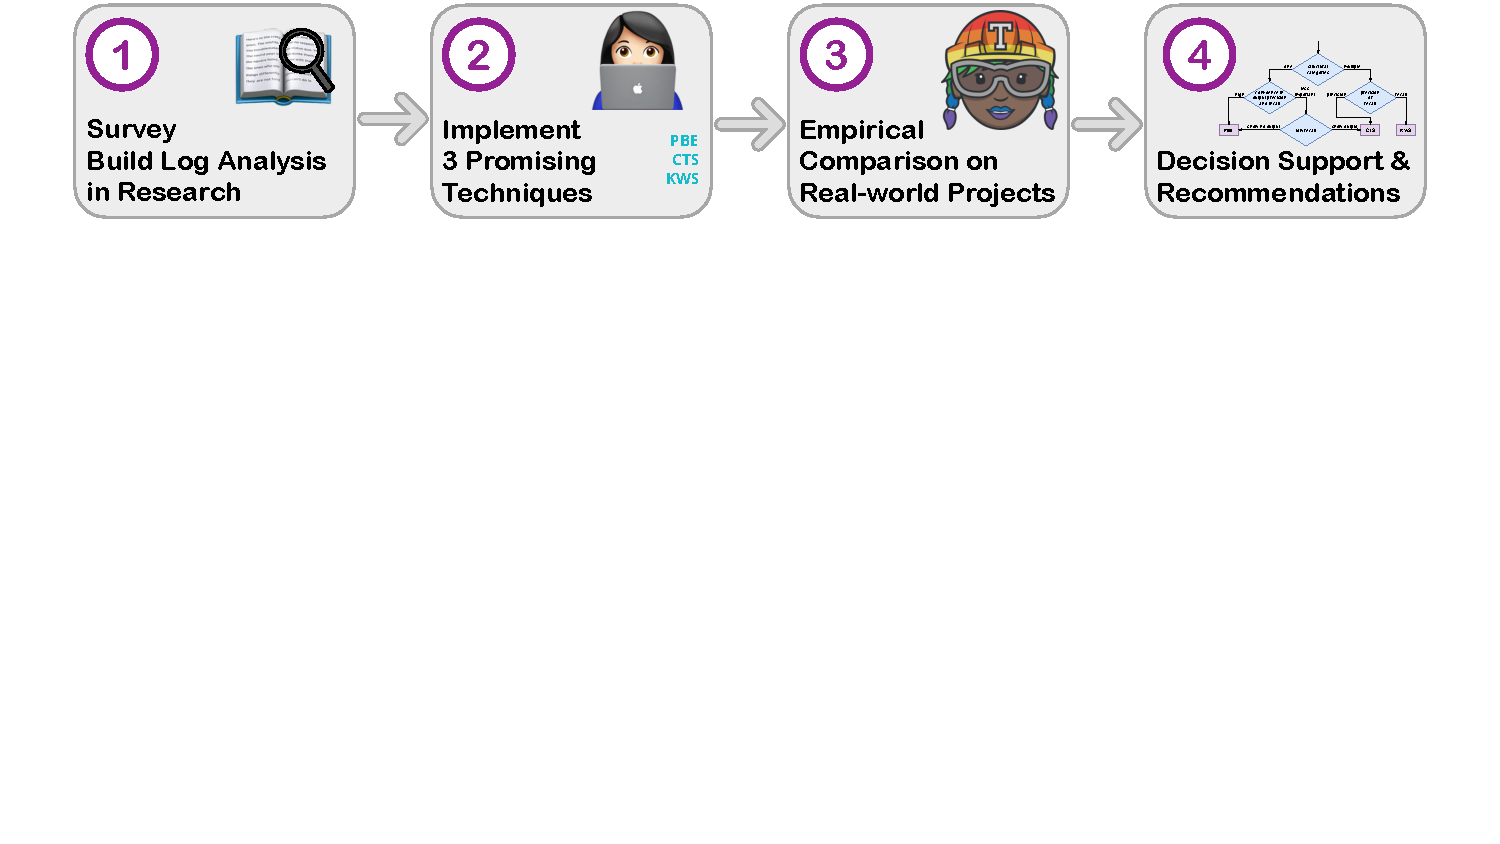
\includegraphics[width=\textwidth, trim={1.2cm 10.5cm 1.2cm 0cm},
	clip]{img/overview.pdf}
	\caption{Research Design.}
	\label{fig:overview}
\end{figure*}

Despite its central role in helping developers and in enabling
novel, on-ward processing applications,
the process of how to
automatically analyze build logs has thus far not been systematically
overviewed as a research topic, bringing us to the first
research question:
\begin{simplebox}[minipage boxed title*=-5cm]{\textbf{Research Question
1}}
What is the state-of-the-research on analyzing build logs?
\end{simplebox}

To answer this question, we start our investigation---pictured in
\Cref{fig:overview}---with an
extensive literature study (step 1).
The literature
survey identifies various strategies to
analyze build logs, among which are developing
custom parsers, using regular expressions, doing manual inspections,
searching for keywords, or performing natural language processing.
However, there is currently no guidance on when to use which of these
approaches.
Unfortunately, our survey also shows that
less than half of the 61 works which rely on build log analysis
describe it in sufficient detail and that
the few available implementations are all based on either a custom parser
or regular expressions.
These two approaches in particular are problematic, as their creation
and maintenane is manual and expensive, does not generalize across build
logs from different build environments, and is, as the experience of
TravisTorrent has shown, prone to error.
In fact, some even ``strongly discourage'' the creation of such
bespoke parsers~\cite{urli2018design}.
In summary, the outcome of our literature survey shows the need for a new
generation of automated techniques to analyze build logs, which are
documented in detail and which are openly available, together with
guidance on when to use which tool.

%Using 1) a set of
% manually curated regular expressions,
% similar to TravisTorrent~\cite{beller2017oops},
% 2) information
% retrieval techniques,
% % Can you shortly explain the technique here?
% and 3) a list of search keywords
% to identify regions of interest in the build log.

%% \begin{itemize}
%%   \item \textbf{(referred to as PBE)}
%%   Based on manually supplied example pairs of build logs and chunks,
%%   PBE automatically synthesizes
%%   a regular expression extracting the given chunks within the build
%% logs.
%%   % these second sentences about what the techniques stand for could
%%   % also be merged to a paragraph after the itemize
%%   PBE mimics regular expressions and parsers while
%%   simplifying their development.
%%   \item \textbf{Common Text Similarity (CTS)}
%%   Text similarity is a common information retrieval technique.
%%   CTS selects lines of a log which are
%%   most similar to the lines present in manually supplied example
%% chunks.
%%   As a common information retrieval technique, our text similarity
%%   approach stands for the machine learning approaches identified in
%%   the literature survey.
%%   \item \textbf{Keyword Search (KWS)}
%%   KWS finds fitting passages by searching the whole
%%   text of a build log for
%%   the occurrence of specific trigger words.
%%   Keyword Search was explicitly mentioned by several articles in the
%%   literature survey.
%% \end{itemize}



% TODO caro: maybe convert this into a proper ordered list?
To fill this gap, we adapted and implemented three novel, prototypical
implementations to
automatically analyze build logs.
The ideas behind the implementations are based on promising approaches
adopted from other research fields and automatic build log analysis
techniques:
a technique 1) able to automatically synthesize regular expressions,
called \emph{Program Synthesis by Example (PBE)}, 2) based on information
retrieval, using \emph{Common Text Similarity (CTS)}  and 3)
inspired by the manual adhoc-search for key parts in the log, employing
\emph{Keyword Search (KWS)}.
These three approaches---regular expressions, text similarity,
keyword search---
have different strengths and weaknesses.
As a consequence,
in the second research question we ask:

\begin{simplebox}[minipage boxed title*=-5cm]{\textbf{Research Question
2}}
How do build log analysis techniques compare?
\end{simplebox}

To answer this question, as a third step,
we conduct an empirical study assessing the performance
of these chunk retrieval techniques in
real-world projects under a variety of conditions.
Our study is based on the \emph{LogChunks} data
set~\cite{brandt2020logchunks}, which encompasses 797 build logs from
80 popular open-source projects and a broad range of different
build tools and programming languages.
Our results show that there is no technique that in general outperforms
the others.
However,
% TODO Caro: 1-2 sentences about results, inclduing some accuracy measures

Finally, due to this ambiguity, we develop a set of guidelines
(\Cref{fig:overview}, step 4)
on how to choose the most suitable build log analysis
technique for the task at hand.
We recommend PBE for use cases where the desired information is always
represented in the same structural way and high confidence in
precision and recall of the chunk retrieval is required.
The results PBE produces are suited for automatic on-ward processing.
CTS is
well-suited when the representation of the desired information varies
slightly and the output of the chunk retrieval is further processed by
a human.
In cases where the textual representation of the desired
information in the log is unpredictable or varies greatly, KWS seems
to be the best choice.
However, its low precision---it extracts a
context of multiple lines around a finding---makes it generally
unsuited for automatic on-ward processing.
Instead, KWS requires a human
to further inspect and interpret the output chunk.
A hybrid solution combining the three techniques might be the best
all-round solution.
Finally, we give a roadmap to guide future research in the field
of build log analysis.

In short, this article contributes
\begin{itemize}
\item the first systematic study of the emerging field of build log
analysis.
\item three prototypical open-sourced implementations of
promising chunk retrieval techniques.
\item a large empirical study comparing the three techniques.
\item systematic guidelines on when to use which technique.
\item a detailed research map to inspire future contributions to the
field.
\item a replication package~\cite{brandt2020chunk-replication}.
\end{itemize}

\section{Systematic Literature Mapping Survey}
\label{sec:survey}

In this section, we survey the emerging field of build log
analysis.
We start with a differentiation to the field of
system log analysis.
% ref to fig 2 so it can be here and above fig 3
Then, we describe the methodology (\Cref{fig:lit-survey})
and results of a systematic mapping
study to
determine the state-of-research on build log analysis following the
guidelines by Petersen et
al.~\cite{petersen2008systematic,petersen2015guidelines}.
We close by summarizing how build logs are commonly
analyzed in literature and discuss the implications of these findings.

\begin{figure}[tb]
	\centering
	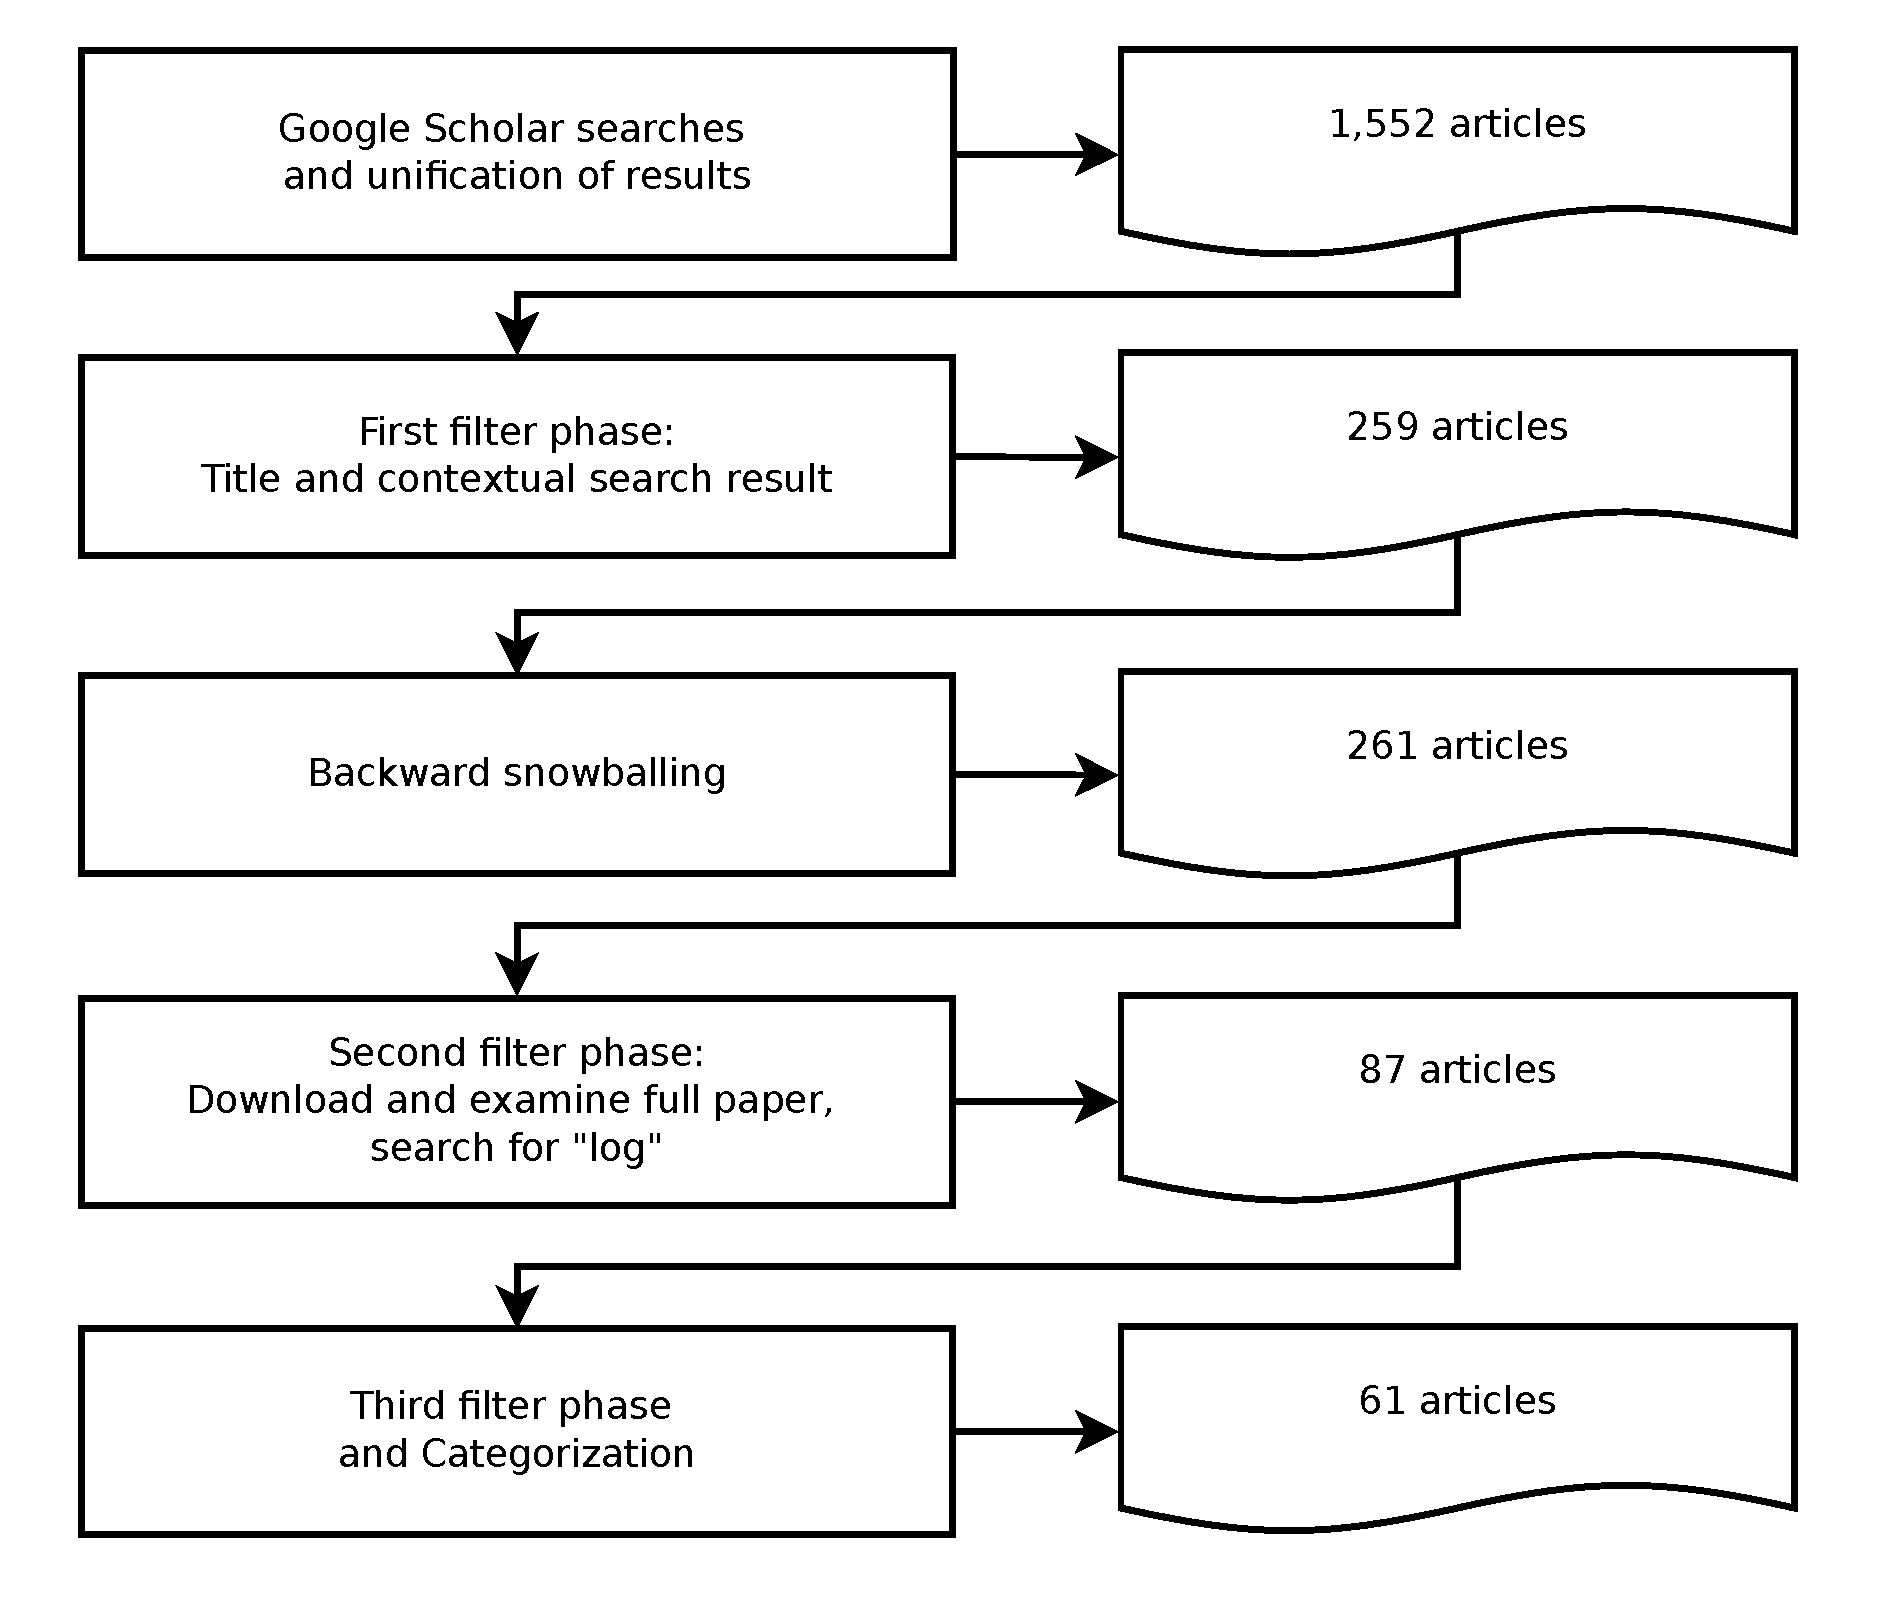
\includegraphics[width=\columnwidth, clip]{img/lit_survey.pdf}
	\caption{Literature selection process, following
	\cite{petersen2015guidelines}.}
	\label{fig:lit-survey}
\end{figure}


\lstset{
  morekeywords={INFO, WARN, 2008, 11, 09},
  alsoletter=-20819,
  keywordstyle=\bfseries\color{Plum},
  escapeinside=**
}
\begin{figure}[b]
  \centering
  \lstinputlisting[breaklines=true]{listings/syslog.txt}
  \caption{System Log excerpt.
Example adapted from~\cite{he2017towards}.}
  \label{lst:system-log}
\end{figure}

\subsection{Distinction from System Log Analysis}
\label{sec:system-log-analysis}
A field related to build log analysis is the analysis of system
logs which are produced during runtime of the system.
The first difference is that build logs are produced during runtime
of the build of the system, not during runtime of the system itself.
In terms of the contents of the logs, the main difference is that system
logs are fundamentally structured
through events.
Each line in a log file represents one event with a
set of fields: timestamp, verbosity level, and raw message
content~\cite{he2017towards}.
\Cref{lst:system-log} depicts two
examplary lines from such a system log.

The first goal in analyzing system log files is generally to
separate the constant and variable parts within a log
message~\cite{nagappan2010abstracting,he2017towards}.
Next, the log
messages are clustered into log events, unifying messages with
identical constant parts and varying parameters.
Then, a log parser works on this intermediate representation.
Its output is an ordered list of timed events and their corresponding
parameter values~\cite{he2016evaluation}.
This structured log can serve as input to various machine learning and
data mining processes.

Some of the techniques developed to parse system logs can operate
on build logs as well, such as methods to retrieve the
values of variable parts in a log message, e.g.\, by using regular
expressions~\cite{nagappan2010abstracting,xu2009detecting}.
% This is the easiest example matching here
% amar et al are not in our literature survey
However, almost all of the techniques developed to analyze system logs
leverage their inherent event structure.
Build logs generally lack this structure and thus require different
bespoke approaches.
% if included: this explanation is not understandable.
% It needs to better embedded in the surrounding text
% One example is comparing execution traces to reference
% traces of intended behavior to detect anomalies.
% Amar et
% al.~\cite{amar2019mining} employed a similar approach to detect
% relevant lines in build logs.
% In this article, we focus on extracting a single specified information
% from the build log as a whole with chunk retrieval techniques.
% Chunk
% retrieval techniques are used as a part of log parsing

\subsection{Literature Selection}
The first step in a systematic literature study is to
establish which works one wants to cover and how to find
them~\cite{kitchenham2009systematic}.
Since the field of build log analysis is relatively young, we
surveyed as broad a population of scientific material as possible.
We did not limit the sources to specific Software Engineering
venues~\cite{petersen2015guidelines}, but included all sources
monitored by Google Scholar, including Bachelor's theses, Master's
theses, and academic slide decks.
We use Google Scholar as opposed to Scopus or
other databases because it is the search engine for scholarly material
with
the broadest and most current index, including preprints.

\Cref{fig:lit-survey} gives an overview of the study selection
process.
An initial Google Scholar search for variations of ``build log''
returned more than 2.2 million results on the 15th of March 2020, many
of which stem
from unrelated fields such as construction or wood working.
We refined the search criteria to exclude such obvious
non-related fields and to exclude works on systems
or event logs (see \Cref{sec:system-log-analysis}).
This left us with 1,552 search results.
% Our replication package documents the full search
% queries~\cite{brandt2020chunk-replication}.
To make handling so many search results feasible, we employed a
three-pass filtering strategy:

First, we filtered articles based on (a) their title and (b) the
contextual information Google Scholar displayed on its search results
overview page.
We included works at large that seemed to bear a resemblance to software
engineering and building software.
Following Kitchham's protocol~\cite{kitchenham2009systematic}, we excluded
works written in a language unintelligible to the authors
(i.e., not English or German), which disregarded fewer than 1\% of search
hits.
We then unified
the results of the four search queries based on the link as the
identifying element, removing 60 articles that appeared in more than
one search query.
We removed further duplicates based on the title and were
left with 256 (16\%) of the original search results.
% removed duplicates of data extraction pass already here

With these 256 remaining articles, we followed a backward snowball
sampling for related work.
If an article referenced a new work in the context
of build log analysis, we added the new one to the literature set.
This added five articles (eight before
duplicate elimination), leading to a total of 261
works.

Second, we performed a finer filter phase by (1) reading their abstracts,
and (2) downloading the
full text of the works and searching the
full text
for the occurrence of ``log.''
If a work showed traces of
working with build logs, we included it for the next filter phase.
In total, we
were left with 87 works after the second filtering phases.

Third, since we had been careful to include rather than exclude borderline
works, a deeper evaluation excluded another 15 articles from the 87
works left after the second filter phase.
Multiple articles were extensions of others.
Of these, we only considered the earliest article which reported on
the analyzing of build logs.
This excluded another 11 articles.
In sum, we extracted data from 61 articles.

\subsection{Literature Classification}
Having trimmed down the set of articles by 95\%, we investigated the
remaining ones in-depth.
We wanted to characterize how research works with build logs.

% TODO	everything is in passive in the following
Specifically, we were interested in
\begin{itemize}
  \item what information is retrieved from the logs and
  what the retrieved information is used for (\textbf{RQ1.1})
  \item which techniques are used to process the build logs,
  in how much detail they are described, and whether they are published
  as tools (\textbf{RQ1.2})
  \item what kind of build logs are used and the origin of these
  logs.
(\textbf{RQ1.3})
\end{itemize}

This lead us to the following research questions:
\begin{simplebox}[attach boxed title to top center={yshift=-6mm}]
{\textbf{RQ1:} What is the state-of-the-research on analyzing build logs?}
% M: All of these are passive
% C: it says resolved, but they still are?
% M: Only the first one still is (don't know how to convert it),
% the others
% are not?
% I exchanged 'extracted' with targeted / analysis
% 'information retrieved' or 'information extracted' will give us
% this is not IR neither IE discussions again
\begin{itemize}[leftmargin=1cm]
  \item[\textbf{RQ1.1:}] What information is targeted in build logs?
  \item[\textbf{RQ1.2:}] Which analysis techniques exist?
  \item[\textbf{RQ1.3:}] Which kinds of build logs are subject to
  analysis?
\end{itemize}
\end{simplebox}

To support the data extraction we created a template that we filled out
for each of the 61 works.
The template contained questions to answer RQ 1.1 through RQ 1.3,
for example ``Is the technique explained in detail?'' and
``What is the source of the build logs?''
As recommended by Petersen et
al.~\cite{petersen2015guidelines}, we started the mapping study with a
pilot:
both authors extracted data from the same five articles and held a
consensus meeting to unify their understanding
of the data extraction template.
We divided the remaining 56 articles evenly between the two authors
and inspected each articlex as closely as necessary to fill out the
template
with confidence,
starting from occurrences of ``log'' or ``build'' within the article's
text.

For questions that did not require a boolean answer, we allowed assigning
multiple tags or categories as the first part (``preparation phase'')
of a virtual open card sorting~\cite{zimmermann2016card}.
An example for this is the question ``What is the source of the build
log?'',
where we assigned tags such as ``Travis CI,''
``Industrial,'' ``Google,'' or
``self-built.''
Once we had classified all works, we went into the second phase of
card sorting
(``execution phase''), in which we grouped tags
together and found synonyms.
% the following adds to the example but is maybe unneeded / too much
For instance, in the case of the build log source we grouped
``Travis'' and ``Travis CI'' together and assigned ``Industrial'' to
all articles that used build logs provided by a company.
The replication package contains the data extraction template and all
results of this step~\cite{brandt2020chunk-replication}.


\subsection{Results}
\addtolength{\tabcolsep}{-5pt}

In this section, we give a general overview over our paper population
and then present the results of the analysis phase of the literature
mapping along RQ 1.1 through RQ 1.3.


\subsection{Descriptive Study Statistics}
To be done.
% TODO moritz: age of papers (graph), kind of
% publication (master, paper)
% published (y, n)


\subsubsection{What information is targeted in build logs? (RQ 1.1)}
\label{sec:rq11}
\begin{figure}
\centering
\begin{subfigure}[t]{\columnwidth}
		\centering
		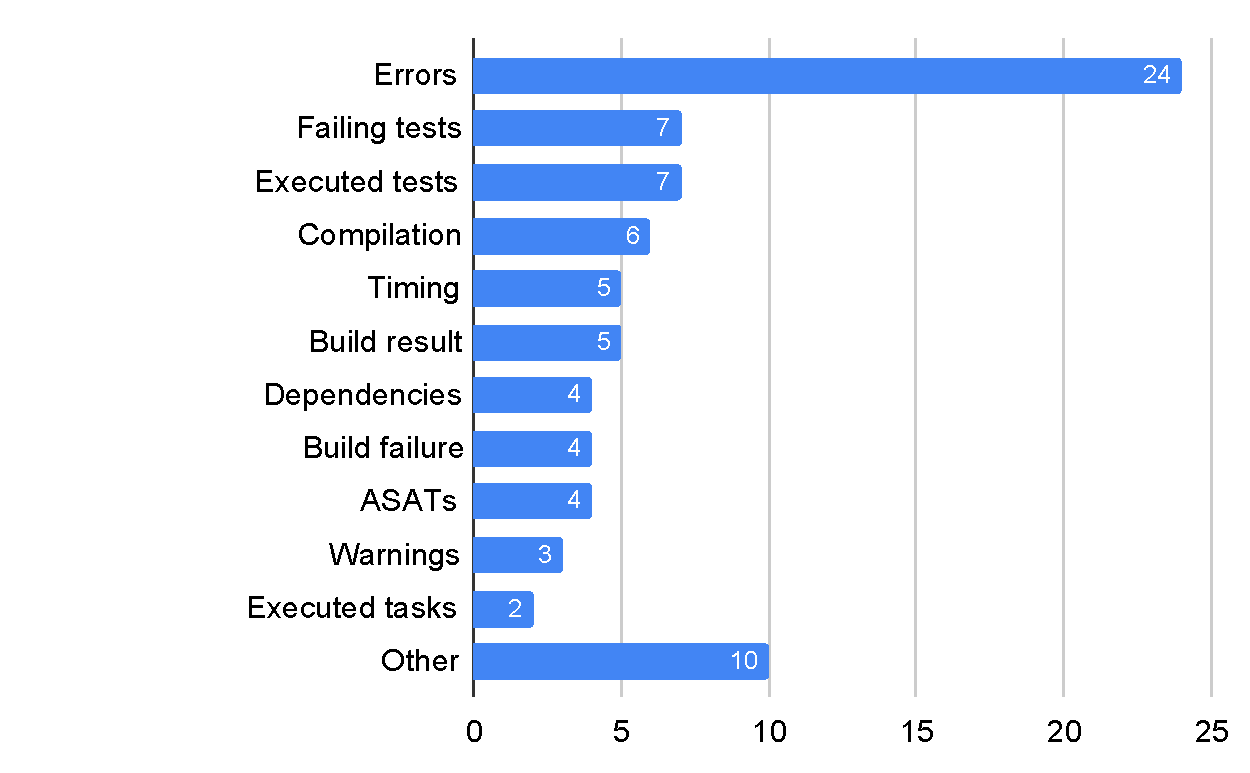
\includegraphics[width=\columnwidth,
		clip]{img/lit-sur/info_target.pdf}
		\caption{Information targeted in build log analysis.}
		\label{fig:litsur:info_target}

\end{subfigure}\hspace{\fill}
\begin{subfigure}[t]{\columnwidth}
		\centering
				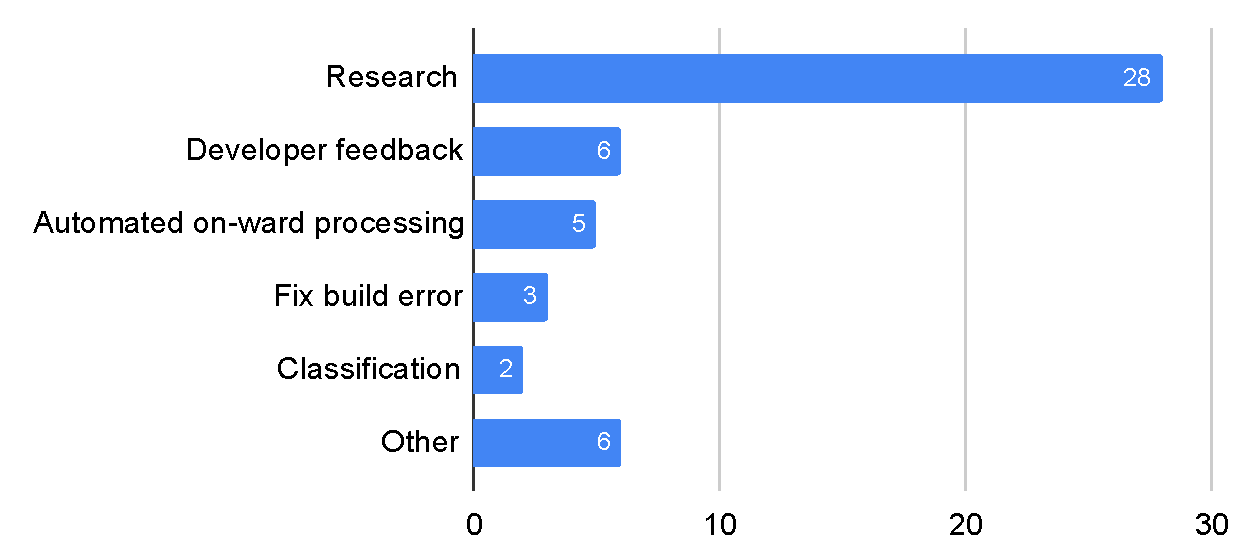
\includegraphics[width=\columnwidth,
				clip]{img/lit-sur/use.pdf}
		\caption{Purpose of build log analysis.}
		\label{fig:litsur:use}

\end{subfigure}

\caption{Multi-label categorization of the 61 relevant articles.}
\label{fig:litsur_r}
\end{figure}

In this section, we describe what sort of information papers usually
extract from build logs, along the results depicted
in \Cref{fig:litsur_r}.

\Cref{fig:litsur:info_target} gives an overview over the frequency of
the targeted information.
The precise information targeted in the build logs varied from article
to article, with a relatively long tail.
Most prominent was the search for errors (39\%), followed by extracting
the executed or the failing
tests (both 11\%).
There were also numerous works which targeted more specialized
information, such as the environments used during the
build~\cite{zolfagharinia2017not}, packages
installed~\cite{selberg2012use}, or hints to source files which
relate to build failures~\cite{ren2018automated}.

\Cref{fig:litsur:use} shows the reason for the
investigated articles to analyze build logs.
The majority of articles (46\%) used the outcome of their build log
analysis to drive further research.
Seo et al.~\cite{seo2014programmers}, for example,
categorized the types of compile errors encountered at
Google.
Other articles (10\%) used the gained insights to give feedback to
developers.
For 8\% of the articles was the retrieved information the input
to a next automatic on-ward processing step:
articles chose
tests that should be part of a reduced but still effective test
suite~\cite{shi2018evaluating} or filled a data structure with
build information, an information source for further tools aiming
to fix a failing build~\cite{vassallo2018un-break}.

% TODO Moritz: add missing figure
We also identified the type of information which the articles
retrieved from the build logs.
In most cases (51\%), the researchers retrieved a chunk of text.
They scanned build logs for compilation
errors~\cite{clemencic2014new} or
the duration of tasks within the build~\cite{zhang2016android}.
36\% of the articles classified the build logs into categories.
For instance, they distinguish failures caused by developers from
failures caused
by infrastructure errors~\cite{lindqvist2019detection} or
determine whether projects use automated static analysis
tools~\cite{kavaler2019tool}.
Other types of information (e.g.,\ counting
lines, summarization) were only retrieved
in one case each.

\subsubsection{Which analysis techniques exist? (RQ 1.2)}
\begin{table*}[tbhp]
\tinyish
\centering
\caption{Overview of build log analysis techniques.}
\begin{tabularx}{\textwidth}{@{}lXl@{}}

\toprule
Name			     & Sources	& Frequency	  \\
\midrule

\raisebox{0.8mm}{Parser} &
\raisebox{0.8mm}{
\cite{vassallo2018un-break,zhang2016android,seo2014programmers,hassan2019tackling,hassan2017automatic,chromy2007integration,mesbah2019deepdelta,wen2018blimp,kwon2018prioritizing,adams2007design,rahman2018impact,brandyberry2006continuous,tomassi2019bugswarm,ren2018automated,vassallo2019automated,cavalcanti2019impact,sippola2013qt,felipe2012towards,shi2018evaluating,urli2018design,selberg2012use}
} &

\includegraphics[width=0.55\columnwidth]{img/lit-sur/techniques-no-guidelines-cropped_21.pdf}
\\

\raisebox{0.8mm}{Regular expression} &
\raisebox{0.8mm}{
\cite{beller2017oops,hassan2017change,macho2018automatically,vassallo2017a-tale,lou2019history,hassan2017automatic,rott2019empirische,zampetti2019study,zhao2018comparing,rausch2017empirical,ghaleb2019studying,zampetti2017open,zhang2019large,kavaler2019tool,morris2010experience}
} &

\includegraphics[width=0.55\columnwidth]{img/lit-sur/techniques-no-guidelines-cropped_15.pdf}
\\

\raisebox{0.8mm}{Manual inspection} &
\raisebox{0.8mm}{
\cite{sulir2016quantitative,hassan2017automatic,bouabana2019theory,barinov2017applying,silva2018build,ghaleb2019empirical,marcozzi2019systematic,hukkanen2015adopting,rausch2017empirical,hassan2017mining,zolfagharinia2017not,cassee2019impact}
} &

\includegraphics[width=0.55\columnwidth]{img/lit-sur/techniques-no-guidelines-cropped_12.pdf}
\\

\raisebox{0.8mm}{Machine Learning} &
\raisebox{0.8mm}{
\cite{hassan2017change,lou2019history,lindqvist2019detection,ren2018automated,schulz2017active}
} &

\includegraphics[width=0.55\columnwidth]{img/lit-sur/techniques-no-guidelines-cropped_5.pdf}
\\

\raisebox{0.8mm}{Natural Language Processing}	&
\raisebox{0.8mm}{
\cite{hassan2017change,lou2019history,schulz2017active}
} &

\includegraphics[width=0.55\columnwidth]{img/lit-sur/techniques-no-guidelines-cropped_3.pdf}
\\

\raisebox{0.8mm}{Information Retrieval} &
\raisebox{0.8mm}{
\cite{hassan2017change,lindqvist2019detection,ren2018automated}
} &

\includegraphics[width=0.55\columnwidth]{img/lit-sur/techniques-no-guidelines-cropped_3.pdf}
\\
% TODO: We need to mention in the text describing the Table what we mean
%by ``Analysis''
\raisebox{0.8mm}{Analysis} &
\raisebox{0.8mm}{
\cite{sulir2016quantitative,haghighatkhah2018test,durieux2019critical}
} &

\includegraphics[width=0.55\columnwidth]{img/lit-sur/techniques-no-guidelines-cropped_3.pdf}
\\

\raisebox{0.8mm}{Keyword Search} &
\raisebox{0.8mm}{
\cite{brandyberry2006continuous,zhang2019large,kavaler2019tool}
} &

\includegraphics[width=0.55\columnwidth]{img/lit-sur/techniques-no-guidelines-cropped_3.pdf}
\\

\raisebox{0.8mm}{Scan} &
\raisebox{0.8mm}{
\cite{clemencic2014new,hibbard2001visualization}
} &

\includegraphics[width=0.55\columnwidth]{img/lit-sur/techniques-no-guidelines-cropped_2.pdf}
\\

\raisebox{0.8mm}{Other} &
\raisebox{0.8mm}{
\cite{zhang2016android,hassan2017change,lou2019history,silva2018build,ren2018automated,schulz2017active}
} &

\includegraphics[width=0.55\columnwidth]{img/lit-sur/techniques-no-guidelines-cropped_10.pdf}
\\

\raisebox{0.8mm}{None identified} &
\raisebox{0.8mm}{
\cite{macho2017preventing,felipe2012towards,orellana2017differences,madeyski2017continuous,zhao2017impact,santolucito2018statically,makihara2018multi,mcintosh2012evolution,gallaba2018noise,matthies2016scrumlint}
} &
\\

\specialrule{\heavyrulewidth}{0pt}{2pt}

\end{tabularx}
\label{tab:litsur:techniques}
\end{table*}
\addtolength{\tabcolsep}{5pt}

\Cref{tab:litsur:techniques} presents the techniques that the articles
described for analyzing build logs.
43 of the 61 articles we inspected mentioned how they are analyzing
build logs.
However, only 16 of these described their method in detail.

The most mentioned method (34\%) was using a parser, where we also
included
rather imprecise statements like ``we parse the build logs''
~\cite{rahman2018impact}.
For such imprecise statements it was often not clear if they describe
a complex parser (including a tokenizer, lexer, etc.) or refer to a
simpler parsing tool based on regular expressions.
If we saw evidence for the latter, we assigned the tag
``regular expression'' instead of the tag ``parser.''
25\% of the articles described the use of regular expressions and 20\%
inspected the logs manually.
For example,
Seo et al.~\cite{seo2014programmers} developed a custom
parser to classify error messages, while Vassallo et
al.~\cite{vassallo2017a-tale} analyzed build logs with regular
expressions.
Ghaleb et al.~\cite{ghaleb2019studying} used a compound approach.
They started with manual categorizing build logs and selecting
search strings that identify the target category.
Based on the search strings they created a script that automatically
classifies the remaining logs.
Another 8\% employed machine learning such as natural language
processing or information retrieval techniques.


Only 25\% of the articles claimed their implementation is available.
Moreover, we
saw some reuse of the few available build log analysis tools.
Five articles employed the tools used to create
\emph{TravisTorrent}~\cite{beller2017travistorrent,beller2017oops,
orellana2017differences,zhao2018comparing} or
an updated version of them~\cite{rott2019empirische,
shi2018evaluating}, two used the
\emph{Maven Log Analyzer}~\cite{macho2018automatically,gallaba2018noise},
and
another two
\emph{MAKAO}~\cite{wen2018blimp,adams2007design,adams2007makao}.

\subsubsection{Which kinds of build logs are subject to
  analysis? (RQ 1.3)}
\Cref{fig:litsur:log_producer} shows the distribution of supported
build tools.
Of the articles we surveyed, 30\% analyzed
Mave~\cite{maven2019website},
16\% analyzed Gradle~\cite{gradle2020website},
and 10\% analyzed Ant build logs~\cite{ant2020website}.

A large amount of the articles analyze build logs
from a small number of build tools.
In most cases, this is because the format of build logs changes
~\cite{staahl2014modeling} and
therefore \textbf{``parsers must be specialized to each build and test
framework''}~\cite{tomassi2019bugswarm}.
Sometimes, aspects separate from the build log analysis motivate
the limitation to a specific build tool.
For example, Shi et al.
focussed on Maven
build logs because they also chose the PIT tool to calculate coverage
and mutation score~\cite{shi2018evaluating}.
PIT is only available as a Maven plugin.

Only 7\% of the proposed methods claimed to be language-agnostic, while
several described they are covering multiple source build tools.
The majority of articles (42\%) used logs from a source that no
second article
targeted.
In 38\% of cases, the articles collected build logs from Travis
CI~\cite{travisci2019webpage};
18\% of the articles processed logs from TravisTorrent; and 8\% included
build logs from industrial projects.
The number of logs analyzed varied greatly between the articles
and we were not always able to
extract it confidently.
23 of the articles analyzed more than a thousand build logs, some
investigated up to 122 million logs.
Of the surveyed articles, 31\% claim to have published their data to
enable further research.
However, we found no clear reuse of build log data sets with the
exception of TravisTorrent~\cite{beller2017travistorrent}, which
Vassallo et al.~\cite{vassallo2017a-tale},
Ghaleb et al.~\cite{ghaleb2019studying},
and several other articles studied.

% TODO Caro: adapt as discussed
% TODO: I think the axes labels are also unncessary for this graph.
%Our other graphs in the lit survey do not have them, either.
\begin{figure}[tbhp]
		\centering
		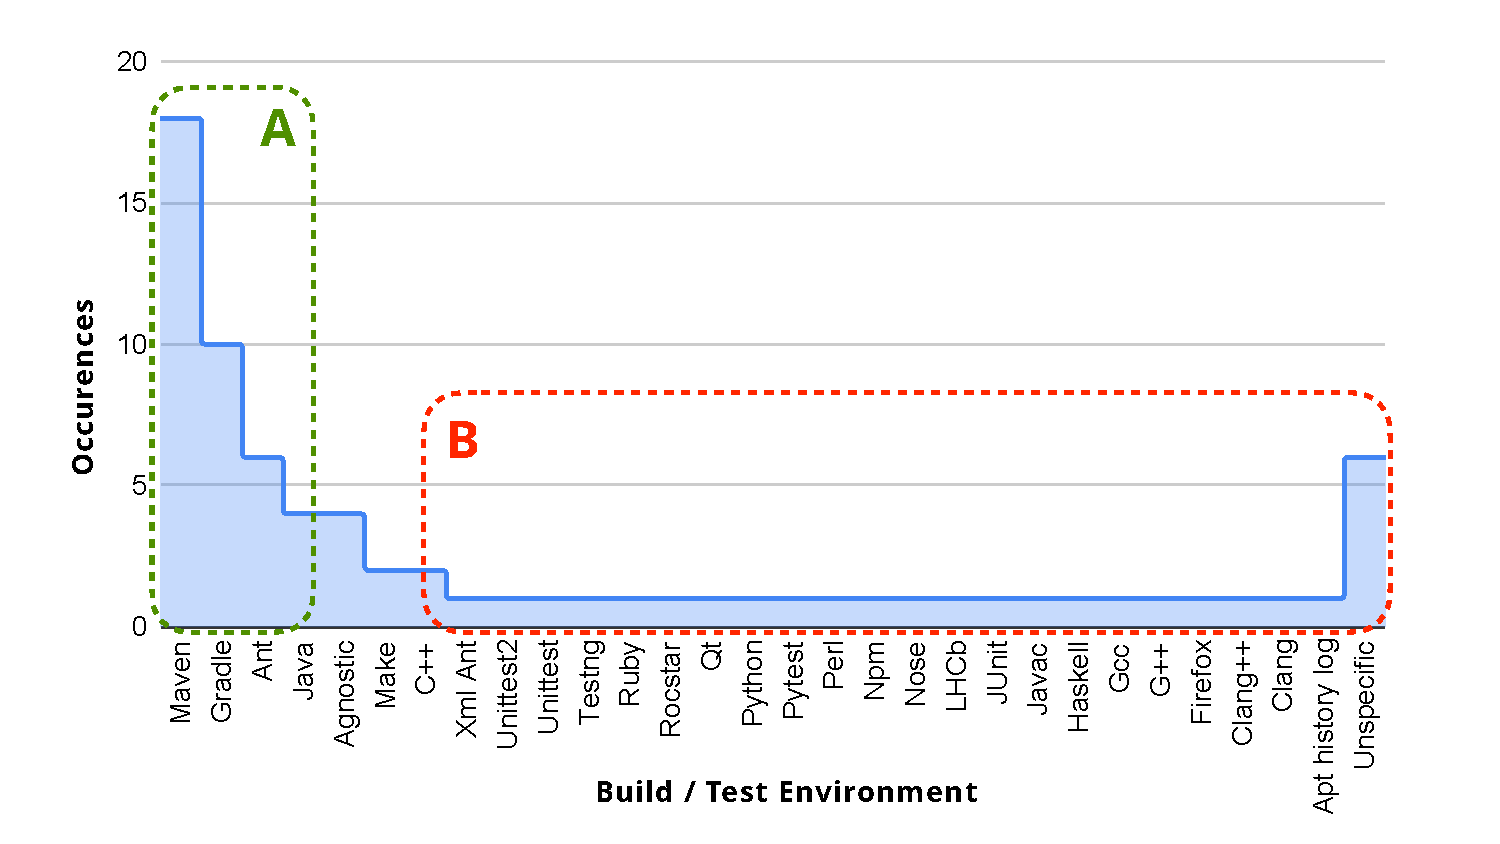
\includegraphics[width=\columnwidth, trim={1.1cm 0.4cm
		1.5cm 0.5cm},
		clip]{img/lit-sur/log_producer_annotated.pdf}
		\caption{Frequency of supported log producers.}
		\label{fig:litsur:log_producer}
\end{figure}


\subsection{Discussion}
\label{sec:lit-sur:discussion}

Our literature survey shows that despite its relatively young age
(first mentioned in a paper in 2001, vast majority after
2016), \textbf{build log analysis is an established technique}
in the literature, with 61 articles making use of it.

% TODO we are extracting failures in the following studies, which is
%mainly what
% literature does, too, right? Highlight here and mention later again

% TODO: this section is crucial.
% maybe we can highlight important findings, by categorizing them either
% as further subsubsections or making it bold in the text?

We saw that various researchers analyze build logs, often because the
logs are the only available source for the
information they need for their studies~\cite{ren2018automated,
seo2014programmers,beller2017oops,zampetti2017open,rausch2017empirical}.

\textbf{most analysis aims to find out why the build failed}

\textbf{most techniques retrieve chunks from build logs}

\textbf{Most log analysis is automated.} Automated approaches are
necessary as many studies target a large number of builds.
Articles
which explicitly mention a manual analysis of the logs, mostly
restrict their work to few logs or take a ``representative sample to
make manual analysis feasible''~\cite{zolfagharinia2017not}.
\textbf{Developing automated analysis tools requires a lot of effort.}
Urli et al.~\cite{urli2018design} strongly discouraged from parsing
build logs for information as it is ``too error prone,'' other
articles pointed to the effort of developing a custom tool.
Regular expressions are known to be tedious to
maintain~\cite{michael2019regexes}.

We observed \textbf{very little reuse of build log analysis tools.}
This can stem from the
high specialization of the developed tools in regards to supported
% TODO: build environments is used a bunch (also in the following), but
% never defined.
build environments and targeted information.

% TODO: draw a conclusion together with figure 5: if reuse were higher,
%lots of effort could be saved?
Several articles noted the variety in log formats for different build
environments, which requires customizing build log techniques for
every supported build environment.
% The following two sentences are passive, however flipped around
% have a different meaning (we want build env -> study count)
\Cref{fig:litsur:log_producer} shows that only a few distinct
build environments are the target of
many studies and tools (roughly, area A).
The majority of build environments was however only targeted by one
article each (roughly, area B).
From this we follow, that the large tail of
\textbf{seldomly-investigated
environments would benefit from the
existence of a more generic solution.}

% TODO we argue this in the intro!
% problem: we have no data on this
\textbf{techniques vary and seem rather randomly applied}

\textbf{modifying the build output is not helpful}, as well as returning
precise data through other documents than the log.
This requires access to the build configuration, is also specific to
the used build environment and prohibits the analysis of
historical data.

\textbf{TODO embed custom plugin discussion}
% TODO very disconnected here
From this, we follow: 1) there is a niche for custom parsers or even
specialized plugins integrated into the build process to make
post-factum
parsing of logs redundant.
Their advantage is that they can precisely report the information which
is required.
A downside of plugins, which are integrated into the CI flow similar to
Deflaker by Bell et al.~\cite{bell2018deflaker}, is that they are unable
to work on historic
builds, i.e., before the moment they were being deployed and that if
information has not been recorded from the beginning but turns out to
be important, it is impossible to retrieve later.
2) the large tail of seldomly-investigated environments would benefit
from the existence of a more generic
solution.

% We implement build environment agnostic build log analysis
% techniques, which are customized to a specific project by
% the training examples which the user provides.
% In addition, the \emph{LogChunks}~\cite{brandt2020logchunks}
% data set we chose for our evaluation covers a broad range of build
% environments.
% % Further, the training examples also specify the log chunk targeted
% by the
% % retrieval, which enable our chunk retrieval techniques to retrieve
% % a broad range of information from build logs.


% This task of retrieving specific chunks of text from the
% build logs can be solved by the chunk retrieval techniques we compare
% in this article.
% Our results can support researchers in choosing a
% suitable technique for their data set of build logs and the chunks
% they want to retrieve.
% By relieving them from building custom parsers
% we enable them to cover a much wider range of languages and build
% tools in their studies.


\section{Chunk Retrieval Techniques}
\label{sec:techniques}
%TODO here we sell our techniques as superior.
% match in intro?
%TODO: really? currently the discussion does not show this 'need'!
The outcome of our literature survey shows the need for a new
generation of techniques to analyze build logs.
In this section we argue how our research sets the first step to
address this need by introducing three techniques that retrieve
specific substrings (chunks) from build logs.
We present defining characteristics of these so called \emph{chunk
retrieval techniques} and present the techniques we developed in
detail.
% TODO At the end of what?
At the end we illustrate how the techniques operate on a concrete
example and sketch out their implementation.

\begin{table*}[htb]
\centering
\caption{Chunk retrieval techniques.}
\begin{tabularx}{\textwidth}{@{}llXll@{}}
\toprule
Name			     & Acronym & Identification Technique
& Granularity & Configuration \\
\midrule
Program Synthesis by Example & PBE     & Regular expression program
& Character   & In/output examples	\\
Common Text Similarity	     & CTS     & TF-IDF \& cosine similarity,
expected number of lines & Line        & Output examples	   \\
Keyword Search		     & KWS     & Keywords, expected number of
lines			 & Line        & Keywords, context length  \\
Random Line Retrieval	     & RLR     & Random sample
& Line	      & Retrieval length	  \\
\bottomrule
\end{tabularx}
\label{tab:techniques}
\end{table*}

\subsection{The Case for Chunk Retrieval on Build Logs}
In summary, the results of the literature study show the need for
build log
analysis techniques that are \emph{automated},
\emph{agnostic of the build environment}
and can be \emph{configured with little effort}.

% what we need is some derivation of the three techniques 1) regex 2)
%cts 3) kws, best repeated here in the discussion and then from the lit
%survey above, section 2.4.2
For this reason, we are focussing on techniques that run automatically
after being configured through examples or keywords.
\emph{Examples consist of logs and corresponding chunks.}
The user provides these examples and keywords, which are easy to adapt
whenever the user adds new examples.

To analyze build logs,
we propose to use chunk retrieval techniques.
These retrieve a substring,
that describes a specific information, from a build log.
Generally, chunk retrieval techniques
can also be used to classify build logs, e.g.\ by checking
which substring was retrieved.
Therefore, chunk retrieval techniques
cover the great majority of the types of log analysis we saw within
our survey.

We implement three chunk retrieval techniques based on approaches
previously described by several articles:
PBE mimics regular expressions, while simplifying
their development.
We chose text similarity (CTS) as a common information retrieval
technique and implement the ad-hoc approach of
searching for specific strings or keywords within KWS\@.

To evaluate and compare the three chunk retrieval techniques
we create a data set with logs from failed builds and corresponding
chunks that describe error messages or
``the reason the build failed.''
This was also the information
most targeted by the articles in our survey (see \Cref{sec:rq11}).
In addition to that, our data set encompasses a broad range of
build environments which enables us to measure the generic
applicability of the techniques.

% The articles within our study mainly tried to retrieve or classify
% errors or reasons for the build to fail from the logs.
% Therefore we chose the log chunk ``describing why the build failed''
% ~\cite{brandt2020logchunks} for our empirical comparison study
% of chunk retrieval techniques.
% The techniques we implement are in principle agnostic to the targeted
% log chunk, thus we believe our results can be generalized to other
% kinds of log chunks.

\subsection{Characteristics of Chunk Retrieval Techniques}
% TODO Caro: Wouldn't this place perhaps be better to contain
%the pargraph about why chunk log techniques are more general
% than other approaches?

\label{sec:crt-characteristics}
In this section, we formalize our use of chunk retrieval techniques.
By this word, we refer to techniques that automatically
retrieve pieces of information that appear literally in build
logs, i.e., techniques that do not aggregate, combine, or deduct
information.
We call such pieces of information in build logs
\emph{chunks}.
% and the techniques \emph{chunk retrieval techniques}.
The techniques we investigate here do not require a formal lexer and
parser to analyze the entire structure of build logs, but focus on
ad-hoc extracting just one specific piece of information per
configuration.

With the term \textit{configuration}, we abstract over the training
and parametrization that different techniques require in different
forms.
A configuration can be explicitly stated or implicitly derived
by learning through provided examples.
It is therefore a manual
specification of which information the chunk retrieval should target.
It also supplies the necessary information for the technique to
identify the targeted information chunk in a build log.
Each chunk
retrieval technique has a specific \textit{granularity}, i.e.,\ the
smallest piece of text it can return (e.g., a line, or a word).
% The
% granularity might be adjustable by configuration.

\emph{Running a
chunk retrieval technique} means executing a fully configured
technique to consumes as input a build log in plain text format and to
produce an array as output.
The array consists of substrings of the
build log text.
\Cref{tab:techniques} summarizes and distinguishes the techniques
we present along the
characteristics described above.

\subsection{Program Synthesis by Example (PBE)}
The concept of \emph{Programming by Example} aims to capture the
intent of the user through examples which they provide.
Leveraging this approach, we implemented a chunk retrieval technique
for build logs.
The \emph{PROSE library}~\cite{prose2019webpage} is the basis of
our implementation.
This library builds on the generic program synthesis framework
\emph{FlashMeta}~\cite{polozov2015flashmeta:} and the specialized
text extraction DSL \emph{FlashExtract}~\cite{le2014flashextract:}.
Both enable us to synthesize regular expression programs
consistent~\cite{mitchell1982generalization} with a set of in-
and output examples given by the user.
The usage of example enables the user to configure a chunk
retrieval without understanding the whole structure of
the build log.

\subsubsection{Configuration}
In- and output example pairs are the main driver of Programming by
Example; we refer to them in short as \emph{examples}.
The \emph{input} is the text of the build log file.
The \emph{output} is
a substring of the log file text, representing the
substring that the synthesized program should retrieve when
given the corresponding input file.
One or multiple examples, the
training set, \emph{configure} a specific chunk retrieval with PBE:
they define the substring of a build log that should be extracted.
The PROSE program synthesis then tries to construct a program
consistent with all training examples.
If PROSE cannot synthesize a program, e.g.,\
because the regular expression
necessary is too complicated to synthesize, PBE returns the
error message ``no program found.''

\subsubsection{Application}
A run of PBE takes a build log file as input and applies the
synthesized regular expression program.
It then returns the substring
of the build log matched by the program.
% I hope this is fine, you can also cut this sentence if it still
% bothers you :)
If the program finds no match because the analyzed build logs
does not contain the structure defined by the training examples,
PBE returns an error message.

\subsection{Common Text Similarity (CTS)}
Text Similarity approaches are widely used to filter unstructured
textual software artifacts~\cite{runeson2007detection,
marcus2005recovery,antoniol2002recovering,mccarey2006recommending}.
We investigate a chunk retrieval technique that
retrieve those lines from a build log which are most
similar to examples given by the user.

\subsubsection{Configuration}
To configure chunk retrieval through text similarity we chose to use
the same concept of examples as for PBE.
The lines of the output strings of the training examples define the
search query.
We represent each line as a term vector where each entry counts
how often a word appears within the line.
These vectors exist in a space ith as many dimensions as different
words appear in the log text.
This Vector Space Model~\cite{schutze2008introduction} defines
text lines as more similar if they contain the same words in the same
frequencies, meaning their term vectors point in a similar direction
in the vector space.
We use the cosine function to calculate the angle between two
term vectors.
The smaller the angle between term vectors, the more similar are the
corresponding lines.
This is called \emph{cosine similarity}~\cite{korenius2007principal}.

To improve the similarity calculation, we prune very often or
very rarely appearing words.
Finally, the
algorithm weighs the vectors using TF-IDF, a best practice for natural
language queries~\cite{lee1997document}.

\subsubsection{Application}
To retrieve the desired information from a build log, we parse the
whole text and process it in the same way as the search query.
The algorithm calculates the cosine
similarity~\cite{korenius2007principal} to compare each line of the
build log with each line of the search query.
After summing up the
similarities of each build log line to all search query lines, we sort
the build log lines in decreasing similarity.
The average number of
lines in the outputs of the training examples determines how many of
the most similar lines are returned as the output of the retrieval
run.

\subsection{Keyword Search (KWS)}
When developers scavenge for a specific piece of information within a
large amount of unstructured information, a first ad-hoc approach they
use is to search for related keywords.
Indeed, this was one of the
most common approaches we took when searching for the reason a build
failed while creating the \emph{LogChunks} data
set~\cite{brandt2020logchunks}.

\subsubsection{Configuration}
A set of keywords configures the chunk retrieval with KWS\@.
To better
compare KWS with PBE and CTS, we also configure it through examples.
We associate each example with keywords which appear in the targeted
chunk or close to it.

KWS then searches for those keywords which are tied to the greatest
number of examples in the training set.
If several keywords are associated with the same number of training
examples, and no other keywords are associated with more training
examples, KWS searches for all of these keywords.

\subsubsection{Application}
For a retrieval run, we take a whole build log file as input and
search for all exact occurrences of the keywords.
As keywords are
often not directly describing the desired information, but rather
appear close to the desired information, KWS also retrieves the lines
around the found keyword.
The number of surrounding lines retrieved is
the average of lines in the output of the training examples.


\subsection{Random Line Retrieval (RLR)}
\label{sec:expl-rlr}

To fully comprehend how difficult a task build log analysis really
is without any a-priori knowledge, we include a comparison with a
base line of
picking lines randomly from the build log (RLR).
RLR mimics the
situation of guessing blindly which lines are interesting.
The only configuration option for RLR is the number of lines it should
retrieve.
For a fair comparison to the other techniques (whose number of
returned lines is dynamic), we configure RLR to return the average
number of lines in the chunks of the training examples, thus arguably
giving it a slight advantage.

\subsection{Chunk Retrieval Example}
\label{sec:crt-example}

\begin{figure}[tbp]
  \centering
\begin{subfigure}[tbp]{\columnwidth}
  \begin{lstlisting}[breaklines=true,frame=tlr]
FAILURE: Build failed with an exception.

* What went wrong:
  \end{lstlisting}
  \vspace{-\baselineskip}
  \begin{lstlisting}[backgroundcolor=\color{Cerulean!60},breaklines=true,frame=rl]
Could not determine the dependencies of task ':app:jacocoTestDebugReport'.
> Task with path 'testDebug' not found in project ':app'.
  \end{lstlisting}
  \vspace{-\baselineskip}
  \begin{lstlisting}[breaklines=true,frame=blr]

* Try:
  \end{lstlisting}
\end{subfigure}\hspace{\fill}
\begin{subfigure}[tbp]{\columnwidth}
  \centering
  \begin{lstlisting}[breaklines=true,frame=tlr]
FAILURE: Build failed with an exception.

* What went wrong:
  \end{lstlisting}
  \vspace{-\baselineskip}
  \lstinputlisting[backgroundcolor=\color{Cerulean!60},breaklines=true,frame=rl]{listings/chunk1.txt}
  \vspace{-\baselineskip}
  \begin{lstlisting}[breaklines=true,frame=blr]

* Try:
  \end{lstlisting}
\end{subfigure}
  \caption{Two examples of log chunks explaining why an Android
  build failed.}
  \label{lst:chunk-example}
\end{figure}

\lstset{language=caml, morekeywords={StartExtraction, RegexPosition,
RegexPair,
  EndExtraction}, keywordstyle=\bfseries\color{black}, escapeinside=//}
\begin{figure}[tbp]
  \centering
  \lstinputlisting[breaklines=true]{listings/prose.txt}
  \caption{Simplified regular expression produced by PBE when trained
  with examples from \Cref{lst:chunk-example}}
  \label{lst:prose-program-simplified}
\end{figure}

\lstset{
  language=,
  morekeywords={},
  texcl=false
}
\begin{figure}[tbp]
  \centering
  \begin{lstlisting}[breaklines=true,frame=tlr]
=== RUN   TestSeparator
  \end{lstlisting}
  \vspace{-\baselineskip}
  \lstinputlisting[backgroundcolor=\color{Cerulean!60},breaklines=true,frame=rl]{listings/chunk2.txt}
  \vspace{-\baselineskip}
  \begin{lstlisting}[breaklines=true,frame=blr]
=== RUN   TestGenerateHTML
  \end{lstlisting}
  \caption{Example of a log chunk showing a linter error}
  \label{lst:chunk-example-3}
\end{figure}

To illustrate the chunk retrieval techniques further, we want to give
an example of real-world log LogChunks.
\Cref{lst:chunk-example} shows two excerpts
from Android build logs.
Marked in blue are the chunks
which contain the information on why the
corresponding build failed.

When we train PBE with these two examples, it produces
a regular expression program similar to the one presented in
\Cref{lst:prose-program-simplified}.
The retrieval
starts after a colon and a line separator and before a capital
letter.
It ends before two line separators,
which is consistent with the two example
chunks from \Cref{lst:chunk-example}.
This shows, that the characters structuring the text around the chunk are
crucial for regular expressions to identify a log chunk.
In fact, if we add the third example from \Cref{lst:chunk-example-3}
(which has a
different structural representation) to the training set,
PBE is not able to synthesize a program and returns
``\texttt{no program found}.''
We later express this difference in structural representation through
dividing log chunks into \emph{structural categories}.
The chunks from \Cref{lst:chunk-example}
are in the \emph{same structural category}, while the chunk from
\Cref{lst:chunk-example-3} is in a
\emph{different structural category}.
The results of the empirical comparison study on the chunk retrieval
techniques
show that the structural representation of the targeted chunk greatly
influences
the performance of the chunk retrieval techniques.

CTS will rank the lines from an analyzed build log which are most
similar to the chunks in the training examples
from \Cref{lst:chunk-example}.
It will then return the two lines ranked highest, as the chunks in
the training examples have on average two lines.

Keywords that appear close to the chunk within
the build log configure the technique KWS\@.
For the examples from \Cref{lst:chunk-example} these could be
``FAILURE,'' ``wrong,'' or ``failed''.
The example from \Cref{lst:chunk-example-3} could be found
by searching for ``FAIL.''
If we train KWS with all three examples and the aforementioned
associated keywords, it would search for the three keywords from
\Cref{lst:chunk-example}, as they appear twice---most often within
the training set of three examples.

\subsection{Tool Implementation}
For the comparison study, we implemented each of the chunk retrieval
techniques and a unifying interface.
The unified interface is written in Ruby and
calls the separate technique implementations over the command line.
We implemented PBE in C\# based on the Microsoft PROSE
library~\cite{prose2019webpage} and CTS, KWS, and RLR using
R and the {\tt text2vec} library~\cite{text2vec2019webpage}.


% TODO -- this is a wrong title -- !!
% find better one
\section{Empirical Comparison Study}

%Second, What is the difference between Study Process and
% Study Design? Third, the LogChunks section appears out of nowhere
% and is not related to the section title (different abstraction
% level).

\label{sec:study}

To investigate when the chunk retrieval techniques are suited to
analyze build logs (\textbf{RQ2}), we perform an empirical comparison
study on the \emph{LogChunks} data set~\cite{brandt2020logchunks}.
In particular, we are interested in how many examples a technique
should be trained with (\textbf{RQ2.1}),
how similar the structural representation of the targeted log chunks
has to be (\textbf{RQ2.2}), and how reliable the quality of the
produced outputs is (\textbf{RQ2.3}).
This leads us to the following research questions:

\begin{simplebox}[minipage boxed title*=-1.5cm,
attach boxed title to top center={yshift=-6mm}]
{\textbf{RQ2:} How do build log analysis techniques compare?}
\begin{itemize}[leftmargin=1.2cm]
  \item[\textbf{RQ2.1:}] How many examples does a technique need to
  perform best?
  \item[\textbf{RQ2.2:}] How structurally similar do the examples
  need for a technique to be applicable?
  \item[\textbf{RQ2.3:}] How accurate are the retrievals of a technique?
\end{itemize}
\end{simplebox}

\begin{figure*}[tb]
	\centering
	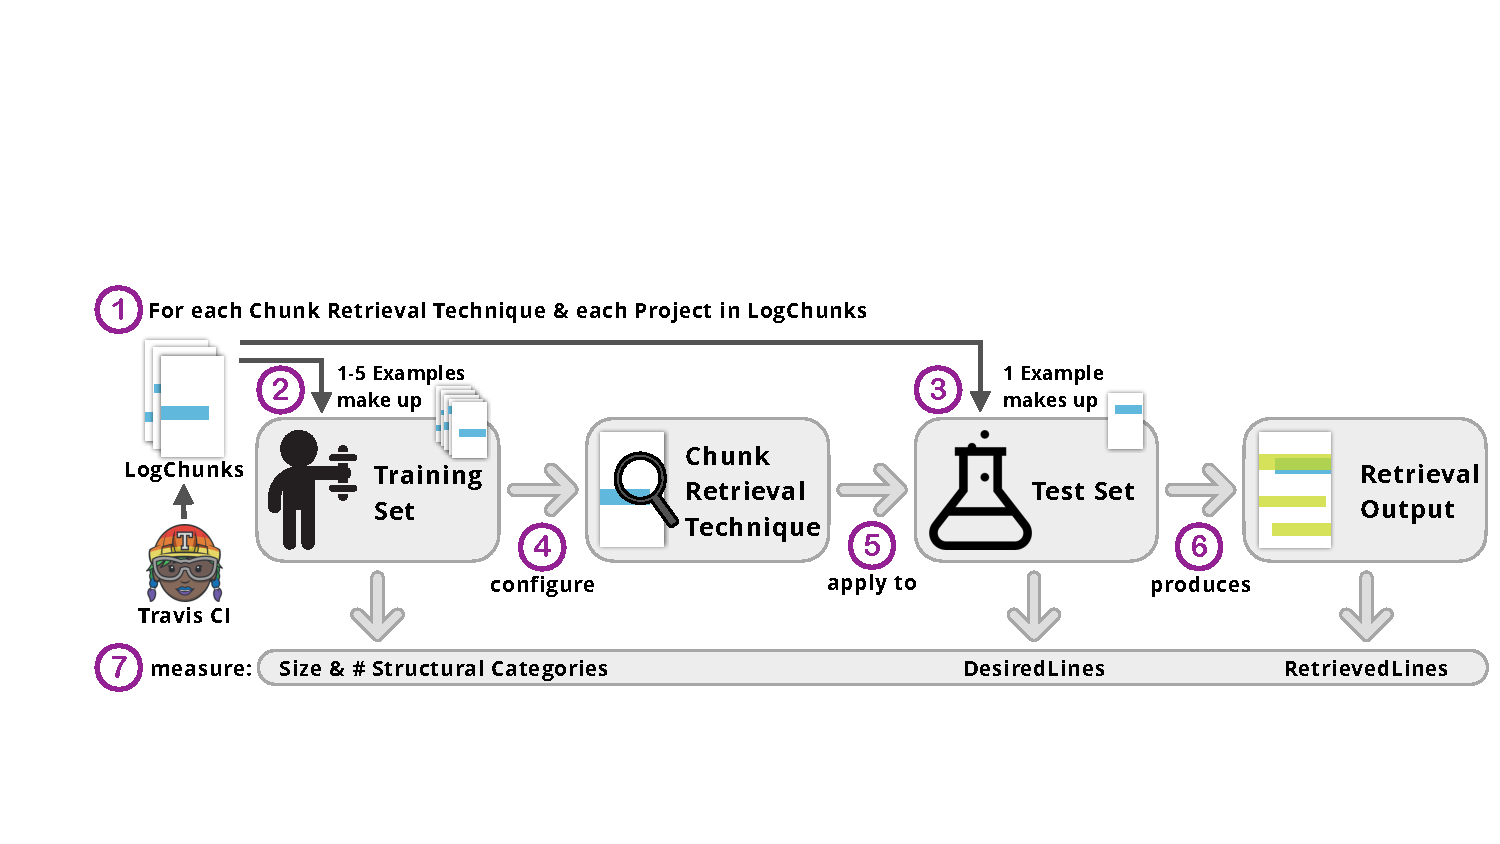
\includegraphics[width=\textwidth, trim={1.6cm 2.5cm 0.2cm 4.8cm},
  clip]{img/study.pdf}
  % TODO wrong caption!!! find adequate one
	\caption{Design of the technique comparison study.}
	\label{fig:study}
\end{figure*}

% TODO this might need some glue / intro text

\subsection{LogChunks Data Set}
\label{sec:logchunks}
To conduct the study in this paper, we created the
\emph{LogChunks} data set~\cite{brandt2020logchunks}.
It encompasses 797 build logs from Travis CI,
stemming from a broad range of 80 GitHub repositories and 29
programming languages.
For each file, we manually ``labeled
the log part (chunk) describing why the build
failed''.
We included keywords, which we
would use to search for the selected chunk within the log.
In
addition, we categorized the log chunks according to their format
within the log.
If the chunks were surrounded by the same markings
within the log, we assigned them the \emph{same structural category},
as described in \Cref{sec:crt-example}.

This, the build log text, the corresponding chunk,
the search keywords, and the assigned structural categories
make up one \emph{example}.
Examples are the basic units in the training and test sets of our
empirical comparison study.

% TODO: find better title!!!!
\subsection{Study Execution}
\Cref{fig:study} gives an overview over the steps within our empirical
comparison study.
In the following, we each of the steps and the metrics
we measure to answer our research questions.

We apply every one of the four chunk retrieval techniques
% TODO Check abstraction level: leave out acronyms?
(PBE, CTS, KWS, and RLR) on all 80 repositories represented in
\emph{LogChunks} \circlenum{1}.
For each repository, we select training sets of size 1, 2, \dots 5
examples \circlenum{2}.
% For this, we select all examples in \emph{LogChunks}
% (as defined in \Cref{sec:logchunks})
% We begin by selecting all examples
% that correspond to one GitHub repository---and thus the
% same build environment (1).
We vary its size to measure how many examples we need to
confidently configure a technique.
The training set is so small because the examples have to be
manually created by a user.
A larger training set would oppose our goal of providing techniques
that can be configured with little effort
(see \Cref{sec:lit-sur:discussion}).
The test set consists of an example based on the build log produced
chronologically after the build logs in the training set \circlenum{3}.
In this way, we train on examples from past build logs and test on
more recent logs.
% We chose a test set size of 1, as users of the techniques
% should receive reliable results on every build log they analyze.
% M: and why is this important? Doesn't everyone want such stability
%of results?
% C: motivation why only one test example.
% we can also leave that out
% and answer if we are asked about it
In the next step, we configure a chunk retrieval technique with
the examples from the training set \circlenum{4} and apply the technique
to the
training set \circlenum{5}, which produces the retrieval output
\circlenum{6}.
Based on this, we collect the following measurements \circlenum{7}:
the size of the training set (\textbf{RQ2.1}),
the number of structural categories in the training
set (\textbf{RQ2.2}),
the lines of the retrieval output ($\mathit{RetrievedLines}$),
and the oracle: the output defined in the test example
($\mathit{DesiredLines}$).
From these we calculate accuracy metrics (\textbf{RQ2.3}):

\vspace{0.2cm}
\begin{itemize}[leftmargin=0.4cm] \itemsep1em
	\item $|\mbox{True\ Positives}| = \mathit{DesiredLines} \cap
	\mathit{RetrievedLines}$ \vspace{0.2cm}\\
	True positives are lines that appear both in the output of a
	technique as well as the chunk defined in the
  test example.

	% What about when a line is replicated twice?
	% I.e., Are line numbers part of this? => no.
	% not checked, but if lines are identical they also contain
	% the same information so if someone asks we can defend I think

	\item $\mbox{Precision} = \dfrac{|\mathit{True\
	Positives}|}{|\mathit{RetrievedLines}|}$ \vspace{0.21cm} \\
	Precision of a chunk retrieval describes which proportion of
	the retrieved lines were actually desired.

	\item $\mbox{Recall} =
	\dfrac{|\mathit{True\ Positives}|}{|\mathit{DesiredLines}|}$
	\vspace{0.2cm} \\
	Recall of a chunk retrieval describes which proportion of the
	desired lines were retrieved.

	\item $\mbox{F$_{1}$-score} = 2 \cdot \dfrac{\mathit{Precision}
	\cdot \mathit{Recall}}{\mathit{Precision} + \mathit{Recall}}$
	\vspace{0.2cm}\\
	In addition, we calculate the F$_{1}$-score, the harmonic mean
	of precision and recall.
  We prefer F$_{1}$ to other aggregate
	measures such as accuracy because for a
	``needle-in-the-haystack'' scenario, we want to avoid bloating
	our results by correctly not finding lots of irrelevant log
	lines.

	% actually that is now giving recall another (nicer) name
	% improved if we just talk about recall later?
	\item Successful retrieval = $\mathit{true}\ \mathit{iff}\
	\mathit{Recall} = 1, \mathit{false\ otherwise}\vspace{0.1cm}$
	Partially Successful retrieval = $\mathit{true}\ \mathit{iff}\
	0 < \mathit{Recall} < 1, \mathit{false\ otherwise}\vspace{0.1cm}$
	Unsuccessful retrieval = $\mathit{true}\ \mathit{iff}\
	\mathit{Recall} = 0, \mathit{false\ otherwise}\vspace{0.1cm}$

	We define a successful retrieval as one where all desired
	lines were extracted, therefore when recall is one.
	A retrieval is partially successful if at least some of the
	desired lines were extracted.
	If the retrieved lines contain none of the desired lines
	a retrieval was unsuccessful.
\end{itemize}

\section{Results}
% TODO check abstraction level: mention PBE, CTS etc?
This section first presents the results for each chunk retrieval
technique separately.
Afterwards, we compare the three techniques with each other and to a
random baseline.

\subsection{Program Synthesis by Example (PBE)}
\label{sec:r:pbe}

\begin{figure}[tbp]
		\centering
		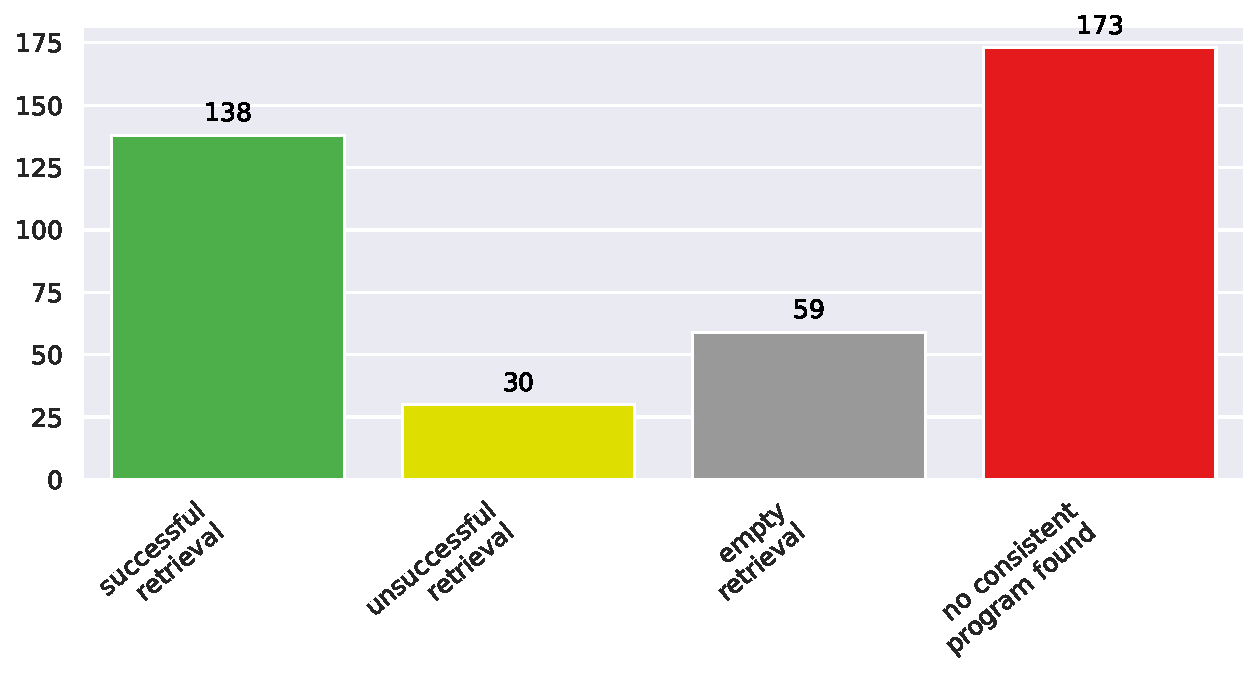
\includegraphics[width=\columnwidth,
		clip]{img/big-study/failure-reason-pbe.pdf}
		\caption{Results of chunk retrieval with PBE.}
		\label{fig:failure-reason-PBE}
\end{figure}

\lstset{
  language=,
  morekeywords={Test, Output, Desired},
  keywordstyle=\textbf,
	frame=single
}
\begin{figure}[!t]
  \centering
\begin{subfigure}[b]{\columnwidth}
  \begin{lstlisting}[breaklines=true,frame=tlr]
[0K$ test/sass-compile-tester.sh
  \end{lstlisting}
  \vspace{-\baselineskip}
  \begin{lstlisting}[backgroundcolor=\color{Yellow!60},breaklines=true,frame=rl]
Error: Invalid CSS after "2.3em": expected expression (e.g.
1px, bold), was ";"
	on line 86 of sass/components/dropdown.
  \end{lstlisting}
  \vspace{-\baselineskip}
  \begin{lstlisting}[breaklines=true,frame=blr]
	from line 5 of sass/components/_all.sass
  \end{lstlisting}
	\caption{Yellow: chunk retrieval output ($RetrievedLines$)}
	\label{lst:pbe-part-success-output}
\end{subfigure}

\begin{subfigure}[b]{\columnwidth}
  \begin{lstlisting}[breaklines=true,frame=tlr]
[0K$ test/sass-compile-tester.sh
  \end{lstlisting}
  \vspace{-\baselineskip}
  \begin{lstlisting}[backgroundcolor=\color{Cerulean!60},breaklines=true,frame=rl]
Error: Invalid CSS after "2.3em": expected expression (e.g.
1px, bold), was ";"
	on line 86 of sass/components/dropdown.sass
	from line 5 of sass/components/_all.sass
	from line 6 of bulma.sass
  \end{lstlisting}
  \vspace{-\baselineskip}
  \begin{lstlisting}[breaklines=true,frame=blr]
  Use --trace for backtrace.
  \end{lstlisting}
	\caption{Blue: targeted chunk ($DesiredLines$)}
	\label{lst:pbe-part-success-desired}
\end{subfigure}
  \caption{Example for a partially successful retrieval
  (PBE retrieved only
  two of the four targeted lines).}
  \label{lst:pbe-unsuccessful}
\end{figure}

\begin{figure*}
\centering
    \textbf{Program Synthesis by Example (PBE)}\par\medskip
\begin{subfigure}[b]{\columnwidth}
		\centering
		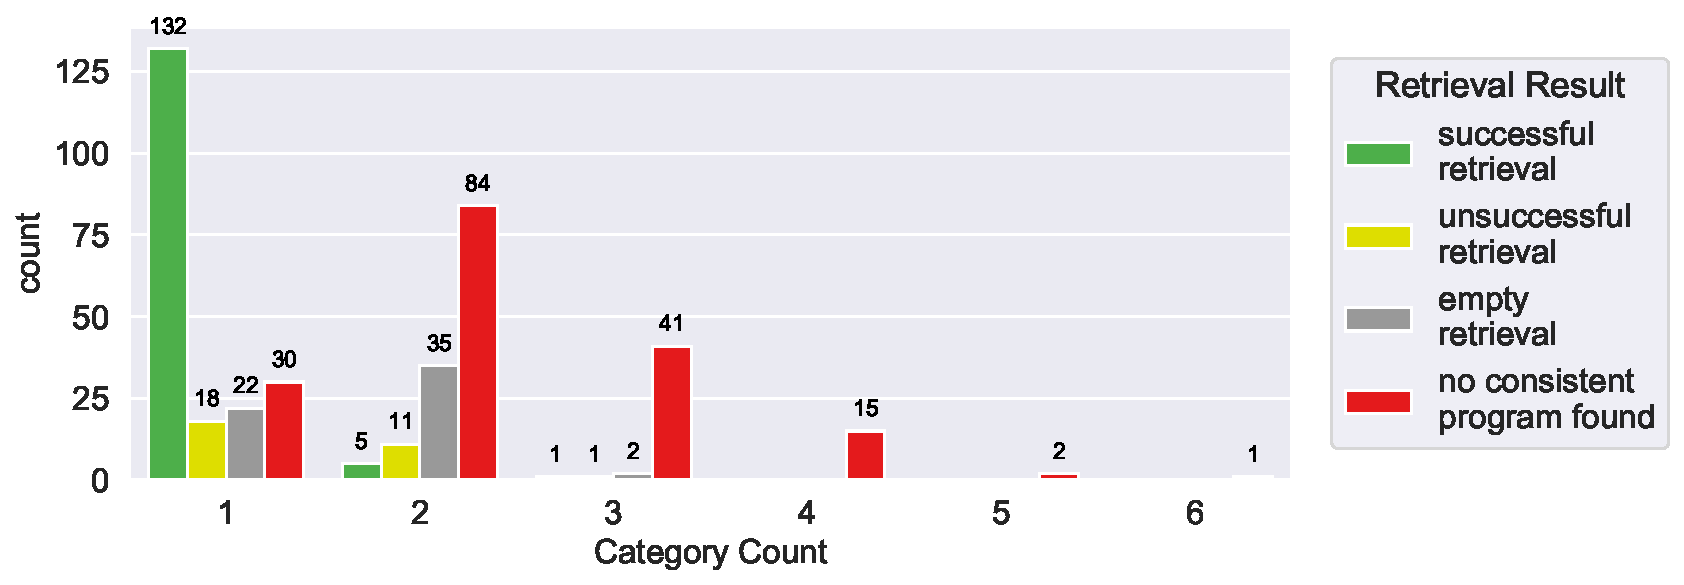
\includegraphics[width=\columnwidth,
		clip]{img/big-study/failure-reason-categorycount-PBE.pdf}
				\caption{Successfulness of retrieval
				compared by structural category count
				in training and test sets.}
		\label{fig:failure-reason-categorycount-PBE}
\end{subfigure}\hspace{\fill}
\begin{subfigure}[b]{\columnwidth}
		\centering
		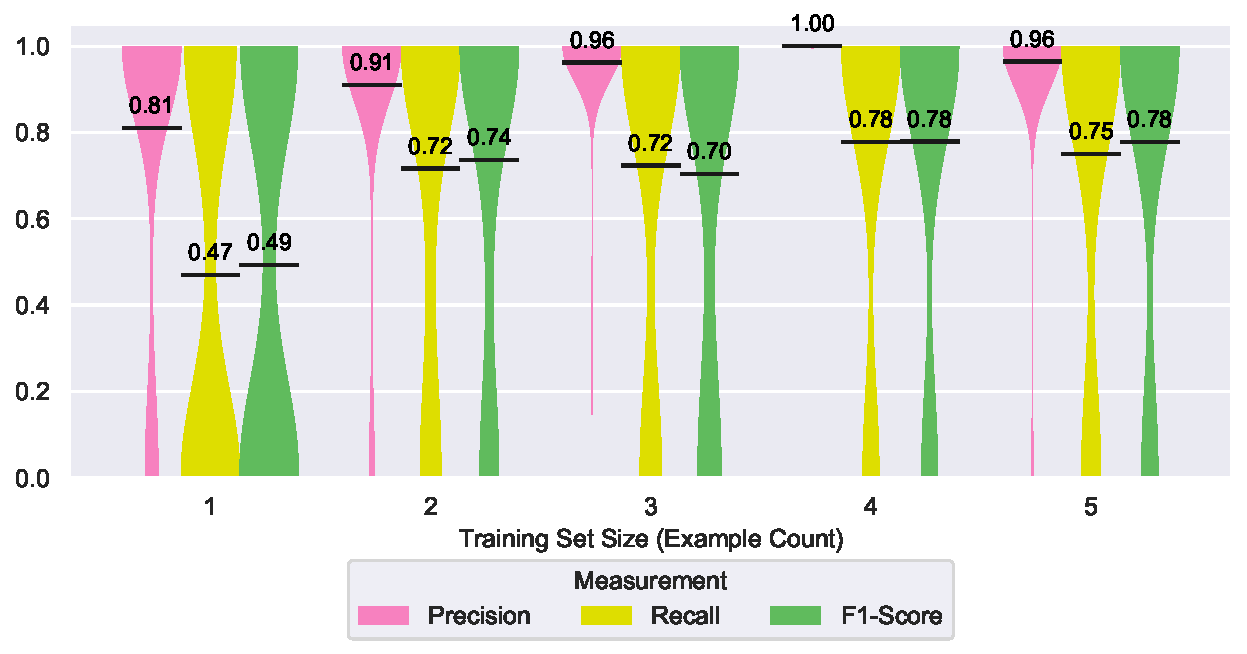
\includegraphics[width=\columnwidth,
		clip]{img/big-study/recall-precision-examplecount-sythesisworked-PBE.pdf}
				\caption{Precision, recall, and
				F$_{1}$-score when PBE could synthesize
				a consistent program compared with the
				size of the training set.}
		\label{fig:recall-precision-examplecount-sythesisworked-PBE}
\end{subfigure}
\caption{Results of chunk retrieval with  Program Synthesis by Example
(PBE)}
\end{figure*}

% actually, we could cut this figure and move it's explanation
% to the next one (this is an aggregation of the next one)
% however, having them separate eases the entry into the results a bit
% and we have explanation of the categories before the more complicated
% aspect of the change with more structural categories
\Cref{fig:failure-reason-PBE} shows the results of chunk
retrieval with PBE.
It shows how many of the retrieval runs were successful or
partially successful, as well as the number of runs where the
synthesized program did not match on the analyzed build log or where
no program could be synthesized.
% The last two results stem from the regular expressions and their
% synthesis, therefore only apply to PBE.
Out of the overall 400 runs, 5 per each one of the 80 example
sets, PBE extracted all desired lines successfully in 138 cases.
In 18 cases, the synthesized program only extracted a
subset of the desired lines, while in 12 cases it extracted none of
the desired lines.
For these 18 partially successful, the average recall
was 47\%.
\Cref{lst:pbe-unsuccessful} shows how an example of such
a partially successful retrieval looks like.
In it, the synthesized program only
retrieved two (\Cref{lst:pbe-part-success-output})
of the four (\Cref{lst:pbe-part-success-desired}) targeted lines.
In 59 cases, PBE could synthesize a regular expression program, though
it did not match on the test build log.
In 173 of the 400 cases
could PROSE not synthesize a program consistent with all of the training
examples.

\Cref{fig:failure-reason-categorycount-PBE} shows how
the results of PBE
runs depend on the number of structural categories in the training and
test examples.
% It shows the categories from above change depending on how many
% structural categories are present.
The figure demonstrates that program synthesis mostly
returns exactly the desired output when there is only one
structural category present in the training and test examples.
However, when
two or more structural categories are simultaneously present,
PROSE could in most cases not synthesize a program.
For four or more present
categories PROSE could never synthesize a consistent program.

Zooming in on only the 227 runs where PBE could synthesize a program,
\Cref{fig:recall-precision-examplecount-sythesisworked-PBE}
presents violin plots of the precision, the recall
and the F$_{1}$-score
of these runs compared with the number of examples in the training set.
The black horizontal lines show the average of these measurements.
When the training set
size increases from one to two, recall, and F$_{1}$-score increase by
about 25\%, precision increases by about 10\%.
For two or more
training examples, recall, and F$_{1}$-score stay around 75\% and
precision around 96\%.

\subsection{Common Text Similarity (CTS)}
\label{sec:r:cts}

\begin{figure*}
\centering
    \textbf{Common Text Similarity (CTS)}\par\medskip
\begin{subfigure}[tb]{\columnwidth}
		\centering
		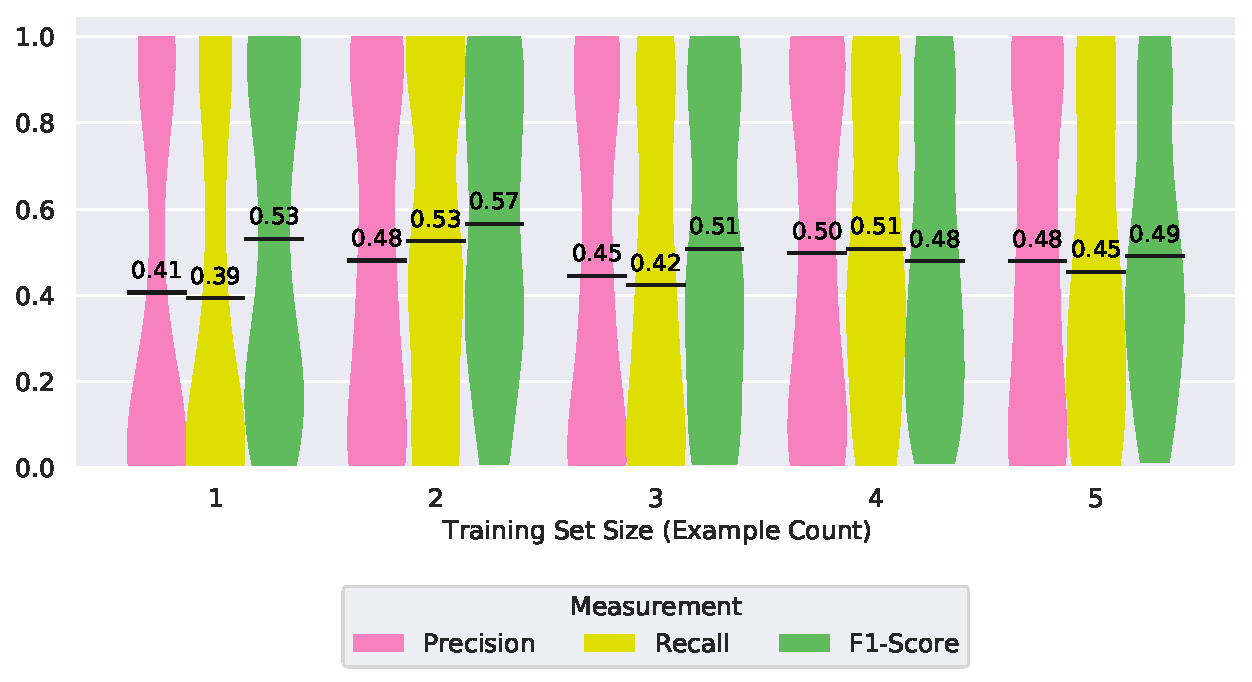
\includegraphics[width=\columnwidth,
		clip]{img/big-study/recall-precision-examplecount-CTS.pdf}
		\caption{training set size.}
		\label{fig:recall-precision-examplecount-CTS}

\end{subfigure}\hspace{\fill}
\begin{subfigure}[tb]{\columnwidth}
		\centering
				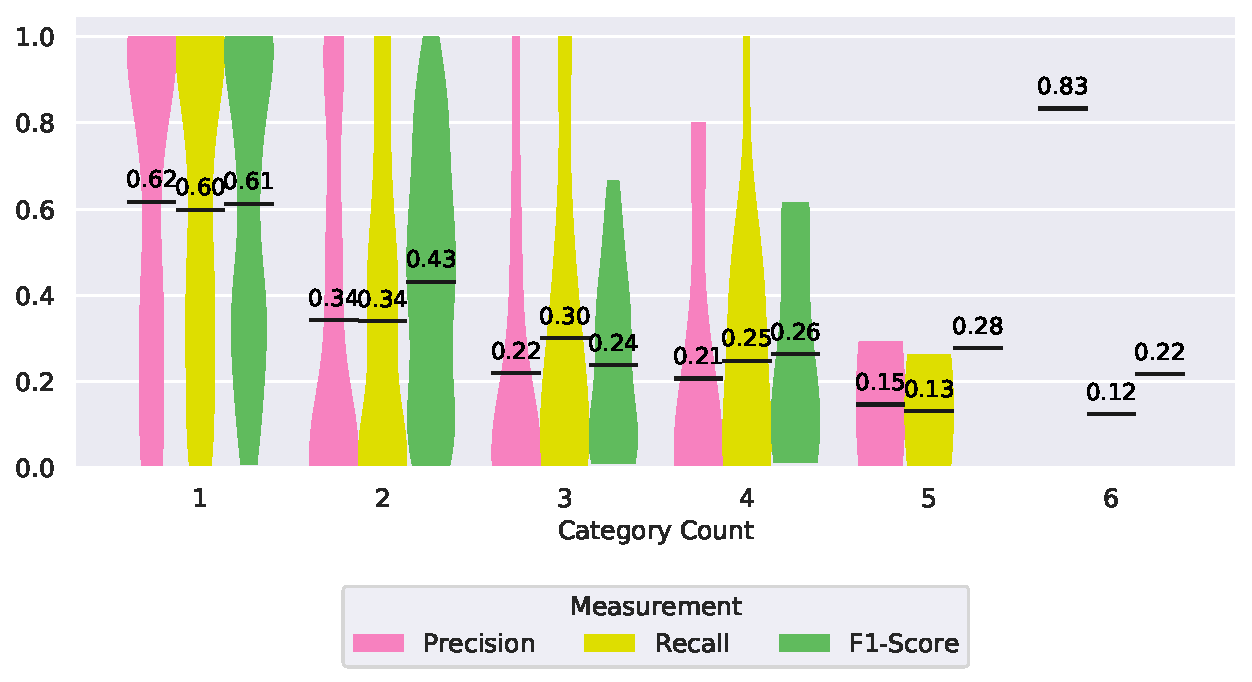
\includegraphics[width=\columnwidth,
				clip]{img/big-study/recall-precision-categorycount-CTS.pdf}
		\caption{structural category count
		in training and test set.}
		\label{fig:recall-precision-categorycount-CTS}
\end{subfigure}
\caption{Precision, recall, and F$_{1}$-score of chunk
retrieval with Common Text Similarity (CTS) compared by \ldots}
\label{fig:results-CTS}
\end{figure*}

% You might even say Figure 12-15 show two
% plots in the short text under the section heading.
% It just makes the
% text flow so much better.

% The following sections are each quite short...
% we could merge them, but then it loses consistency with the other
% result subsections where each plot gets an own paragraph

\Cref{fig:results-CTS} shows violin plots
of the precision,
recall, and F$_{1}$-score of the chunk retrieval runs with CTS.
The black horizontal lines show the average of these measurements.
If the figure shows no violin plot for a category, we only have one
data point or all data points have the same value.

\Cref{fig:recall-precision-examplecount-CTS} presents the
measurements for an
increasing number of training examples.
When using one to five
training examples, the size of the training set has no noticeable
influence on precision, recall or F$_{1}$-score of the chunk retrieval
with CTS.

\Cref{fig:recall-precision-categorycount-CTS} shows the
measurements for an increasing number of structural categories in the
training and test examples.
With increasing category count, precision,
recall, and F$_{1}$-score decrease.
% Especially for more than four
% categories present we have no chunk retrieval runs where all desired
% lines were extracted.

\subsection{Keyword Search (KWS)}
\label{sec:r:kws}
\begin{figure*}
\centering
    \textbf{Keyword Search (KWS)}\par\medskip
\begin{subfigure}[b]{\columnwidth}
		\centering
		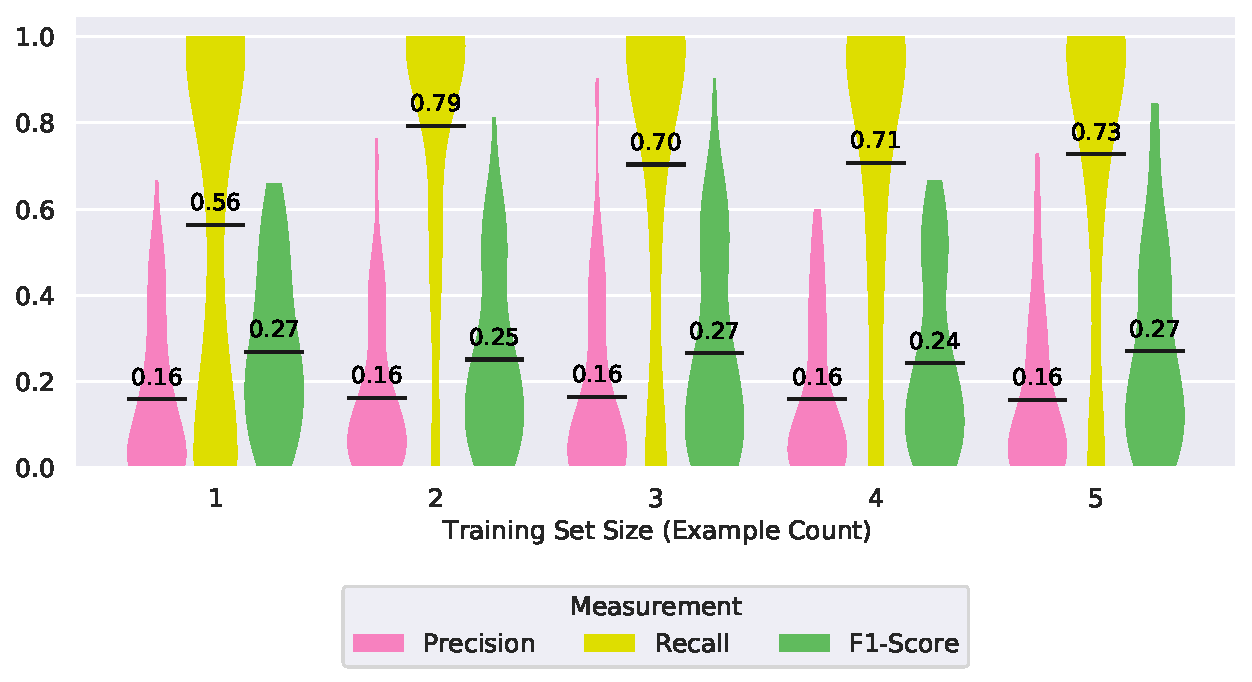
\includegraphics[width=\columnwidth,
		clip]{img/big-study/recall-precision-examplecount-KWS.pdf}
		\caption{training set size.}
		\label{fig:recall-precision-examplecount-KWS}
\end{subfigure}\hspace{\fill}
\begin{subfigure}[b]{\columnwidth}
		\centering
		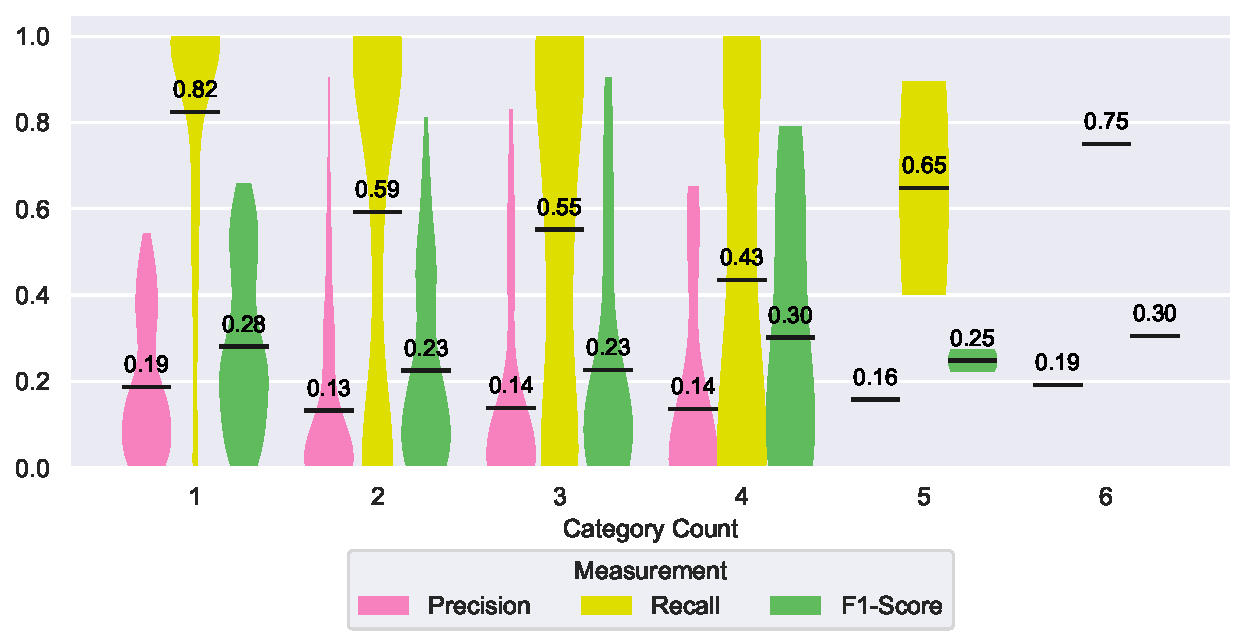
\includegraphics[width=\columnwidth,
		clip]{img/big-study/recall-precision-categorycount-KWS.pdf}
		\caption{structural category count
		in training and test sets.}
		\label{fig:recall-precision-categorycount-KWS}
\end{subfigure}
\caption{Precision, recall, and F$_{1}$-score of chunk retrieval with
Keyword Search (KWS) compared by \ldots}
\label{fig:results-KWS}
\end{figure*}


\Cref{fig:results-KWS} shows violin plots
of the precision,
recall, and F$_{1}$-score of the chunk retrieval runs with KWS.
The black horizontal lines show the average of these measurements.
If the figure shows no violin plot for a category, we only have one
data point or all data points have the same value.

\Cref{fig:recall-precision-examplecount-KWS} presents these
measurements for different
numbers of training examples.
The recall increases by about 12\% when
increasing the size of the training set to more than one example,
while the precision stays constant at around 16\%.
The F$_{1}$-score
stays around 26\%.

\Cref{fig:recall-precision-categorycount-KWS} shows the same
measurements for an increasing number of structural categories in the
training and test examples.
For more than one structural category in
the training and test examples the recall decreases by about 20\% and
the precision decreases about 6\%.
For more than two structural
categories there is no clear trend in precision, recall, or
F$_{1}$-score.

% M: Perhaps, above in our section about logchunks, we would need some
% basic empirical stats -- e.g., how long are the files and how much
% do we usually extract from the log
% C: yup, that would be nice
% sadly, it's quite a bit of work to get those :/
% maybe I/We'll do it at the end
\subsection{Random Line Retrieval}
\label{sec:r:rlr}

The baseline of randomly
picking lines from build logs delivers the expected low and
``random'' results: precision ranges between 8\% and 5\%,
recall between 6\% and 8\%.
As expected, the size of the training set has no impact on precision
or recall of retrieving chunks with RLR.
With a larger number of structural categories within the training and
test sets, the precision of RLR decreases from 7\% to 0\%.
Its recall
increases from 6\%, for one structural category present, to 11\%, for
three structural categories present and drops to 0\% again for more
structural categories.

\subsection{Comparison of All Techniques}
In this section, we compare the results of all four chunk retrieval
techniques and show the impact of structural categories on precision,
recall and F$_{1}$-scores of the different techniques.

% absolute results? is there a nice word for these results
\Cref{fig:success-partial-all} compares the results all of chunk
retrievals techniques in our study.
It shows how many runs per technique were successful, partially
successful or unsuccessful in retrieving the chunk defined in the
test example.
CTS and KWS
extract at least some of the desired lines in 79\% and 88.5\%
of the chunk retrieval runs.
With 38.25\%, KWS also has the highest proportion of fully
successful extractions, followed by PBE with 34.5\%.
PBE has the
lowest number of partial retrievals with only 18 out of 400 chunk
retrieval runs.
All techniques clearly outperform the random baseline (RLR).

\Cref{fig:recall-precision-singlecategory-all,fig:recall-precision-multicategory-all}
show the influence of all training and test examples being from the
same structural category compared to being multiple categories
For more
than one category being present, the recall of PBE decreases greatly.
For CTS and KWS the values also decrease, while RLR is not affected by
the number of structural categories present.
Again, all techniques---except for PBE with multiple structural
categories---yield better retrievals than RLR.

\begin{figure}[!t]
		\centering
		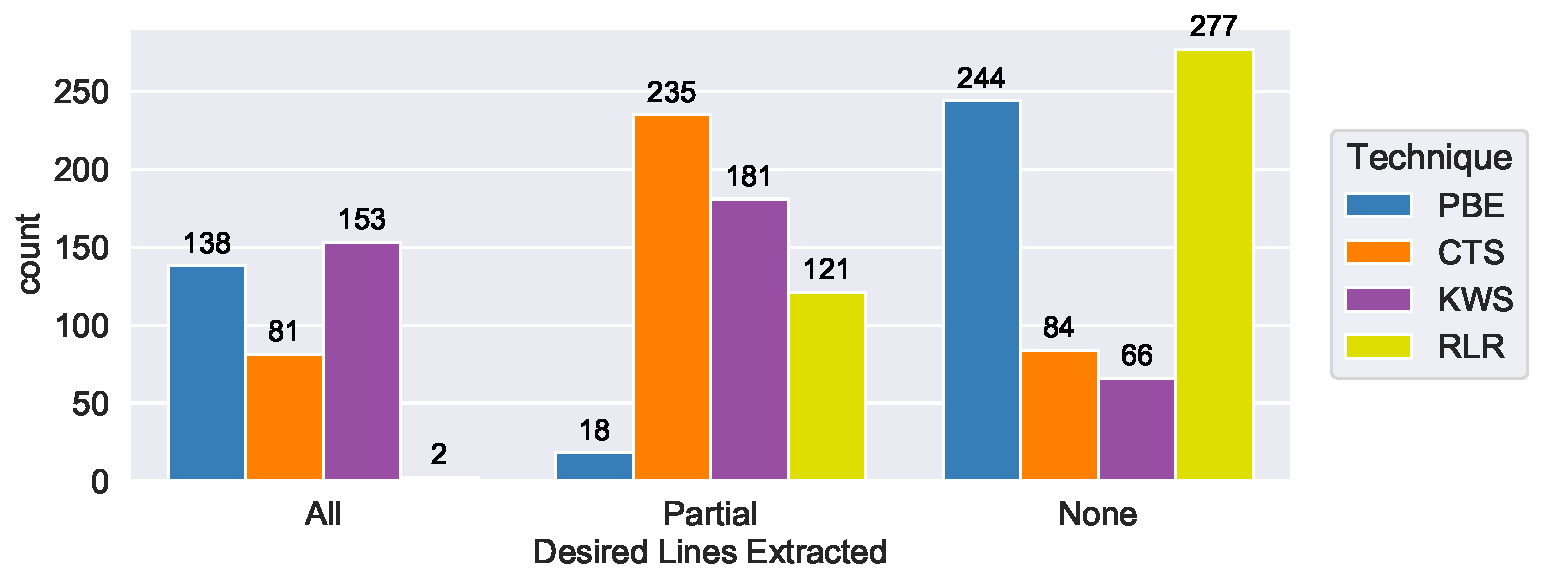
\includegraphics[width=\columnwidth,
		clip]{img/big-study/success-partial-all.pdf}
		\caption{Success of chunk retrievals for all techniques.}
		\label{fig:success-partial-all}
\end{figure}

\begin{figure*}
\centering
    \textbf{PBE, CTS, KWS, and RLR}\par\medskip
\begin{subfigure}[b]{\columnwidth}
		\centering
				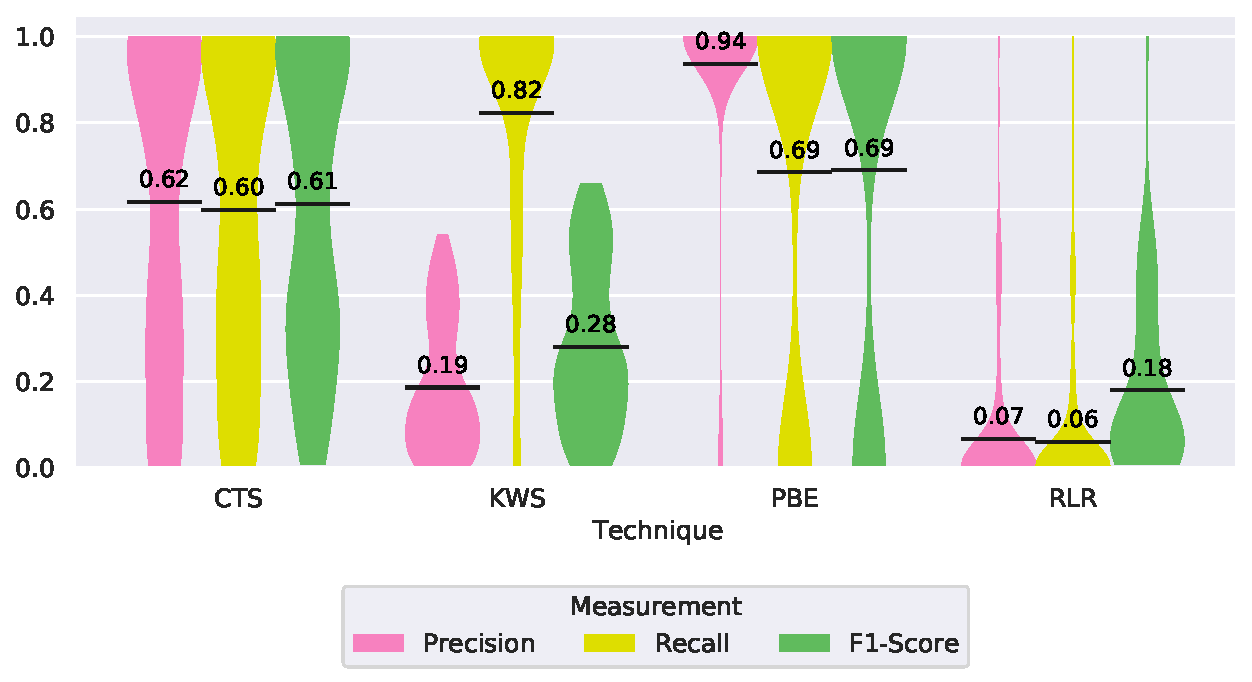
\includegraphics[width=\columnwidth,
				clip]{img/big-study/recall-precision-singlecategory-all.pdf}
		\caption{Training and test examples in 1
		structural category.}
		\label{fig:recall-precision-singlecategory-all}
\end{subfigure}\hspace{\fill}
\begin{subfigure}[b]{\columnwidth}
		\centering
				\centering
		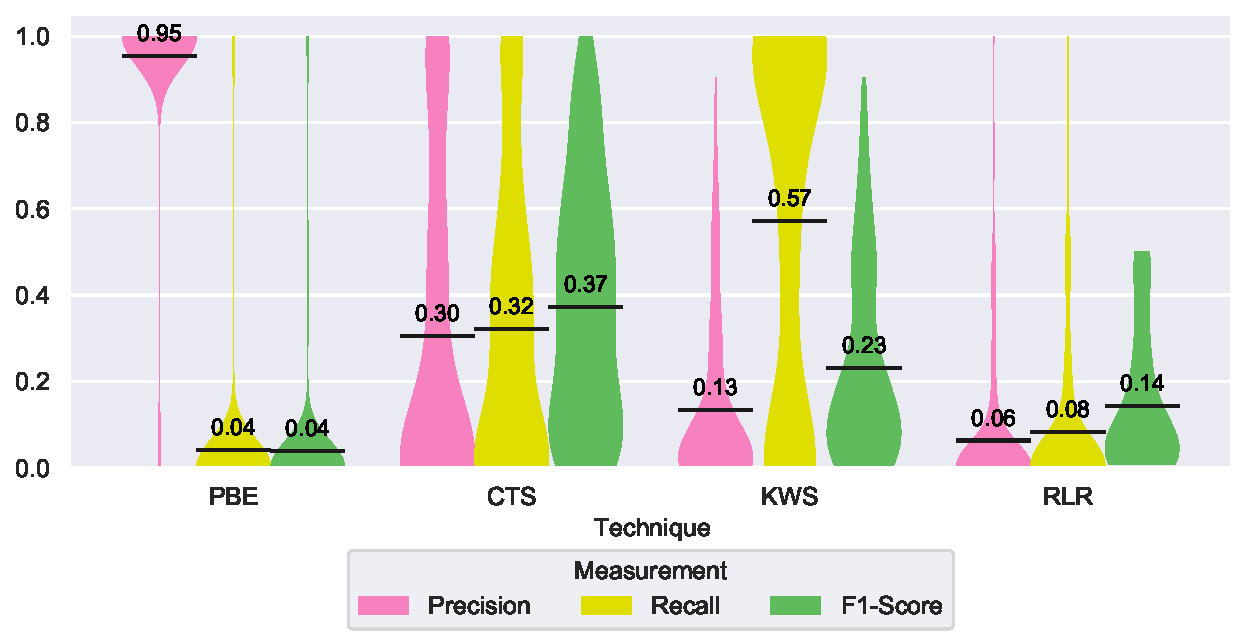
\includegraphics[width=\columnwidth,
		clip]{img/big-study/recall-precision-multicategory-all.pdf}
		\caption{Training and test examples in \textgreater
		1 structural
		category.}
		\label{fig:recall-precision-multicategory-all}
\end{subfigure}
\caption{Precision, recall, and F$_{1}$-score of all
techniques compared, split by structural category count.}
\end{figure*}

\section{Discussion}
\label{sec:discussion}

For the interpretation of the study results, we look at each chunk
retrieval technique separately.
Next, we discuss
which criteria should influence the decision to use a certain
chunk retrieval technique most.
Based on the empirical comparison, we present a
decision tree between the three techniques we investigated.

\subsection{Interpretation of Study Results}
Following from the results of the empirical study,
we give recommendations for
which types of log chunks and how many training examples
each technique is suited, as well as
how their output can be used further.
We summarize these recommendations in
\Cref{tab:single-technique-recommendations}.

% capitalized headings / left title column
% tried it out, I think it looks better with the rest lowercase
\begin{table}[tbp]
\resizebox{\columnwidth}{!}{%
\centering
\begin{tabular}{llll}
  \toprule
  & \textbf{PBE} & \textbf{CTS} & \textbf{KWS} \\
  \midrule
  \textbf{Structural Categories} & 1 & less is better & \makecell[l]{best
  1 \\
  multiple okay} \\
  \midrule
  \textbf{Training Set Size} & 2 & no influence & 2 \\
    \midrule
  \textbf{Precision} & \makecell[l]{high \\ (if synthesis succeeds)} &
  medium &
  low \\
    \midrule
  \textbf{Recall} & \makecell[l]{high \\ (if synthesis succeeds)} &
  medium &
  high \\
    \midrule
  \makecell[l]{\textbf{Confidence in} \\ \textbf{Output Correctness}}
  & high & low &
  \makecell[l]{low (precision) \\ high (recall)} \\	\midrule
  \textbf{Output Consumer} & program & human & human \\
  \bottomrule
\end{tabular}%
}
\caption{Recommendations for each of the investigated chunk retrieval
techniques.}
\label{tab:single-technique-recommendations}
\end{table}

\subsubsection{Program Synthesis by Example (PBE)}

\noindent
\textbf{Configuration and Input.}
The study results show that chunk retrieval with PBE gives best
results when the log chunks are structurally identical.
This is
because PROSE has difficulty synthesizing OR-based
programs~\cite{mayer2015user}.
PBE is thus suited to retrieve information
chunks that always have the same defining surrounding or internal
structure.
To extract for example the reason a build failed, the log
passage describing the failure would always have to start and
end the same way.

When the training examples are of the same structure, one or two
two training examples are enough input for PROSE to synthesize a regular
expression program with good recall.
In the study, additional training
examples from the same structural category
did not improve the chunk retrieval.
In fact, unless they
were in some sense redundant, adding more training examples even
hindered the applicability of PBE.

\noindent
\textbf{Retrieval Output Usage.}
If the program synthesis succeeds and applying the regular expression
program yields an output, PBE has high precision and recall.
The tool
clearly identifies a failing synthesis or when the regular expression
finds no match on a build log.
Therefore, if PBE produces
an output, the user can have high confidence that it is the desired
output.
This preciseness makes output from PBE chunk retrieval
well-suited for machine consumption and therefore automatic on-ward
processing.

\subsubsection{Common Text Similarity (CTS)}
\noindent
\textbf{Configuration and Input.}
Similar to PBE, chunk retrieval using CTS yields better results the
fewer structural categories are present in the training and test
examples.

The number of training examples had no noticeable influence on
precision or recall.
Information retrieval techniques
like text similarity commonly learn on a higher number of examples
than we chose in the study.
Future work should investigate how many
examples yield improvements in the chunk retrieval over a single
training example.

\noindent
\textbf{Retrieval Output Usage.}
CTS has good precision and recall on average, though with a high
variation.
This means that the quality of an output by CTS is hard to
determine, which makes it unsuited for automatic processing and requires
a human to further inspect and interpret the output.
This could include semi-automated procedures such as sending
developers an email with the extracted build failure reason.

\subsubsection{Keyword Search (KWS)}
\noindent
\textbf{Configuration and Input.}
KWS has a higher recall than the two other techniques for multiple
structural categories present in the training and test examples.
This
makes KWS a good technique if there is little prior knowledge of how
the targeted log chunk is represented in the build log.
For the
example of extracting the reason the build failed, KWS is best suited
if a build can fail in various steps logged by different tools and no
pre-categorization of where the build failed is available.

Going from one to two training examples, KWS's recall improves
significantly.
However, further enlarging the training set
does not lead to further improvements.

\noindent
\textbf{Retrieval Output Usage.}
While KWS has the highest recall of all three techniques, its
precision is the lowest.
The output of a chunk retrieval with KWS is
well-suited to be read by humans, but ill-suited for consumption by
automated tools.

\begin{figure}[tb]
		\centering
		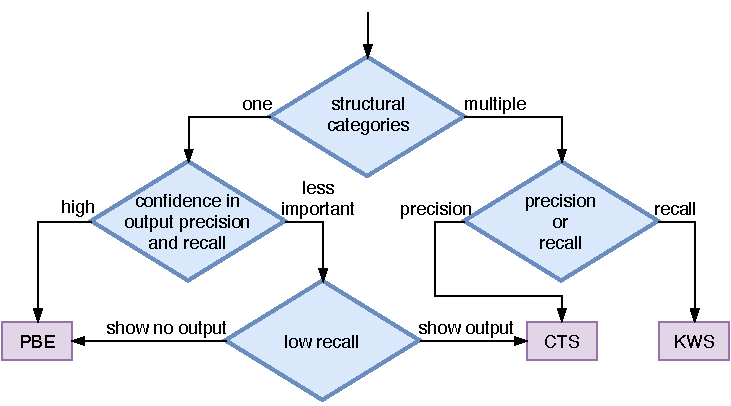
\includegraphics[width=\columnwidth,
		clip]{img/crt-recommendation.pdf}
		\caption{Our decision tree for chunk
		retrieval techniques.}
		\label{fig:crt-recommendation}
\end{figure}

\subsection{Recommendation of Suitable Techniques}
We saw, that each of the techniques is suited for different types of
log chunks and the output of each is suited for different uses.
Now, we unify these results into conditions to answer
our second research questions;
If researchers or developers want to retrieve chunks from build logs,
they can follow these conditions to identify the technique
suited best for their use case.
% I want to ref the figure early bc I believe the text is easier
% to follow when looking at the figure as well
We summarize these conditions in the decision tree in
\Cref{fig:crt-recommendation}.
It is built up of questions
which either lead to more questions or to a leaf node containing a
recommended technique.
At the end of this section we give two concrete examples on how to
apply our decision tree.


% we can't just have a paragraph in a scientific paper start with
% Caveat, I think ;-) Also, we should say why we THINK this is not
%the case.
% Otherwise we weaken our work unduly
% Of course we can! xD
% Agree with the rest.
% It's in TtV, quite close actually
% so I'll comment this out
% also #moreselling :D
% \textbf{Caveat!}
% This is a preliminary hypothesis based on the results
% from our comparison study.
% The recommendations could therefore be
% influenced by idiosyncrasies of our specific implementation of the
% chunk retrieval techniques as well as the \emph{LogChunks}
% data set.

The first and most important aspect that influences a choice for
a chunk retrieval technique are the structural categories.
Are the targeted log chunks always presented in
the same structural way within the build logs? Then the information
chunks in all training examples and the analyzed build log are in the
same structural category.
This is why the first question in \Cref{fig:crt-recommendation} asks
how many structural categories the targeted log chunks have.

If the information chunks are from multiple structural categories
and recall is more important than precision we recommend
to use KWS\@.
If precision is more important than recall, we
recommend CTS, as \Cref{fig:crt-recommendation} shows on the
right half of the decision tree.
We also recommend CTS when the log chunks are
from one structural category, when the user does not require high
confidence in the precision or recall of the outcome and when one
would rather have output with low recall instead of no output at all.
On the leftmost path of the decision tree,
when the representations are from one structural category and the user
wishes high confidence in the correctness of the output or prefers
no output over output with low recall, we recommend PBE\@.

As a final recommendation, one could create a ``super analyzer'' by
combining the different build log analysis techniques studied in this
paper.
Such a super analyzer would likely always first employ PBE
(because of its high accuracy), followed by a combination of CTS and
KWS\@.
Other than initial setup and training time, there is no
downside to this approach if it is implemented in a transparent way to
the underlying technique: the output of the super analyzer could
include from which sub-tool it originated and thus facilitate
automatic on-ward processing or interpretation of the result.


\subsection{Using the Decision Tree}
To illustrate how one would use the decision tree to find a suitable
chunk retrieval technique we describe two concrete examples: a software
team
wanting to monitor their build performance and a
researcher investigating why builds fail.

In the first example, a software development team wants to monitor
the performance of the phases within their CI build.
They are using
Travis CI, which measures the duration of build phases and documents
this within the build log.
As all log statements that report timing
measurements are formatted the same way, the targeted log chunks are
from one structural category.
Therefore, following the leftmost path in
\Cref{fig:crt-recommendation},
the development team should use
PBE to retrieve the duration of a build phase.

In the second example, a researcher wants to investigate whether a small
or large group of test cases
causes build failures.
They gather
CI build logs from various projects.
The task of the researcher is to extract the names of the
failing test cases from each build log.
When they use the
decision tree to select a chunk retrieval technique, they
first have to estimate how uniform the representation of the failing
test cases is in the investigated build logs.
As the researcher is
covering a wide range of test tools, the
log chunks they target are in various, non-predictable structural
representations.
The next question is whether they value precision
over recall.
As they have to manually inspect the results of both CTS
and KWS, they choose recall over precision to avoid having to inspect
the whole log in case the relevant information chunk was not
retrieved.
Therefore, following the rightmost path in
\Cref{fig:crt-recommendation},
the decision tree recommends the researcher to use KWS\@.

In case the researcher wants to avoid manually inspecting the
retrieval results, they have to first separate the CI build logs
according to the test tool responsible for logging the test results.
Then the targeted log chunks are from one structural category and they
can use PBE, trained with examples from each test tool separately.

\section{Threats to Validity}
There are several threats to the validity of the conclusions of our
work.

\textbf{Implementation.}
Our results depend on the implementation of the investigated chunk
retrieval techniques and the libraries we used.
The program synthesis provided by PROSE is the basis for our
implementation of PBE\@.
The
idiosyncrasies of this framework influence the PBE results.
Other
frameworks similar to PROSE might have somewhat different strengths
and weaknesses.
For example, the need for examples from a single
structural category stems from the fact that PROSE cannot learn
regular expression programs with arbitrary boolean conjunctions and
disjunctions~\cite{mayer2015user}.
PROSE introduced this constraint to
keep the synthesis performance reasonable.
At the same time, this is
clearly a current theoretical challenge of all PBE implementations,
and we therefore attribute it to the technique itself, rather than the
specific implementation.

The library
{\tt text2vec}~\cite{text2vec2019webpage}
and the way it splits strings into word tokens is influencing
our implementation of CTS\@.
On the other hand,
{\tt text2vec} is the de-facto standard library to do word embeddings
in R.
We intentionally chose a simple, minimally configured or tuned
approach to compare against.
Tuning the text similarity
meta-parameters more to the specific use case of chunk retrieval from
build logs would yield better chunk retrieval results.

% TODO something like overall, we argue that our implementations and their
% weaknesses stand prototypical for the techniques and tried to limit
% idiosyncrazies as much as possible (give example)

\textbf{Data Set.}
The build logs from the \emph{LogChunks} data set highly affect
the outcomes of the comparison study.
\emph{LogChunks} consists of build
logs from open source projects and therefore it is not clear whether
our results apply to industry projects that use build tools
not popular in open source development.
However, since \emph{LogChunks} covers a wide array of build tools and
programming languages,
we believe that the findings do generalize.
We collected build logs from Travis CI.
Yet, the format of the log chunk we chose
for the evaluation is largely independent of Travis CI\@.
This
is because the reason the build failed is described within the build
logs by the tools themselves and not the Travis CI environment.

\textbf{Training Set Size.}
Especially the results for CTS might be influenced by the fact that we
only trained on one to five examples.
We chose this small training set
size as a user has to provide the training examples
per repository or project and one of the central aims of the chunk
retrieval techniques is that they can be set up wit little effort.
The fact that PBE and KWS performed best with already two training
examples shows that the training set size is large enough to
compare the three techniques.

\textbf{Few Samples with Many Structural Categories.}
Our comparison study shows fewer measurements with many structural
categories than with one structural category category (50.25\% one,
33.75\% two, 13.75\% more than two).
This stems from the fact that we
investigated the chunk retrieval techniques on a real-world data set,
where there were mostly few structural categories within one project.
In addition, the third of the measurements we conducted with two
structural categories already showed the negative effect of an
increasing number of structural categories on the performance of the
chunk retrieval techniques.

\section{Future Work}
% Actually, this future work is very, *very* good.
%It might be
% the best future work I have ever read in an article.
% One idea would be to sell it as such and tie a bit back to our
% first literature survey.
%You can say you give a roadmap to guide
% future research in the field, and sell it in abstract and intro!

There are various future research opportunities based on the
work we presented:

\textbf{Systematic Survey of Industry Approaches for Build
Log Analysis.}
Our survey is limited to academic work and articles.
However, handling build logs is a challenge for a wide range of
practitioners as well.
We propose to investigate the methods used in industry to analyze
build logs.
An example is the Jenkins \emph{build-failure-analyzer}
plugin~\cite{jenkins2020failure-analyzer} or automatically
inferred test results in Azure~\cite{azure2020inferred}.

\textbf{Further Analysis of \emph{LogChunks}.}
We created the
\emph{LogChunks} data set \cite{brandt2020logchunks} specifically for
the comparative
study in this paper, though it can be the basis for various further
analyses of build log data.
The keywords, for example, can be
investigated to answer which keywords are used to search for the
reason the build failed within build logs.

\textbf{Cross-Repository Build Log Analysis.}
We trained and
tested each chunk retrieval technique on examples from the same
repository.
We propose to analyze how techniques could be trained
across repositories, building the cornerstones for build
environment-agnostic analysis tools.
This has the advantage of creating
a default build log analyzer that would work without any pre-training.

\textbf{Comparison with more Chunk Retrieval Techniques.}
This
paper investigates the three chunk retrieval techniques PBE, CTS, and
KWS\@.
Our study design can be reused to evaluate other build log
analysis techniques, such as the parser Tomassi et al.
used to create
BugSwarm~\cite{tomassi2019bugswarm} or the regex-based approach
Beller et al.
used to create TravisTorrent~\cite{beller2017oops}.

\textbf{Refinement of Retrieval Quality for each Technique.} We
investigated basic configurations of existing techniques applied to
chunk retrieval from build logs.
In a next step, each of these
techniques could be refined to better approach the domain of build
logs.
The \emph{LogChunks} data set and our study results act as a
baseline to benchmark such technique improvements.
We propose the
following improvements:
\begin{itemize}[leftmargin=0.4cm]
  \item \textbf{Custom Ranking and Tokens for PBE.} The program
  synthesis through PROSE ranks possible programs according to
  what the user most likely intended.
  One could adapt the ranking
  rules provided by the FlashExtract DSL to fit common build log
  chunk retrieval tasks.
  FlashExtract includes special tokens when
  enumerating possible regular expressions.
  One could extend these
  with tokens found in build logs, such as ``-,''
	``=,'' ``ERROR,''
  or ``[OK''.
  \item \textbf{Meta-Parameter Optimization for CTS.} Information
  retrieval techniques have various meta-parameters which can be
  optimized for the specific use
  case~\cite{panichella2016parameterizing}.
  We propose to further
  investigate improvements in preprocessing of the log text, in
  tokenization of the log lines into terms and in stop words
  lists.
\end{itemize}

\textbf{Usability Analysis of Chunk Retrieval Output.}
Our
analysis of the chunk retrieval output focuses on
precision and recall.
A next step could be to investigate how useful these
outputs really are to developers through controlled experiments or
user studies.

\section{Conclusion}
\label{sec:conclusion-fw}
% TODO CARO conclusion should be a bit longer and a little bit more in
% detail.
 TODO Mention general accuracy measures (techniques performed
up to in F1 score, which is x times better than RLR)
The goal of this paper is to support practitioners and researchers in
their decision on how to analyze build logs.
To this end, we first
conducted a systematic mapping study to map out the available build
log analysis techniques.
We then
implemented three promising chunk retrieval techniques and compared
their performance on the \emph{LogChunks} data set.
Our results show
that the structural representation of the targeted information in the
build logs is the main factor to consider when choosing a suitable
technique.
Secondary factors are the desired confidence in recall and
precision of the produced output and whether precision or recall is
more important for the task at hand.

Finally, we gave an
outline to guide future research efforts in the area of build log
analysis.
Important themes are
% TODO Caro complete :-)




% An example of a floating figure using the graphicx package.
% Note that \label must occur AFTER (or within) \caption.
% For figures, \caption should occur after the \includegraphics.
% Note that IEEEtran v1.7 and later has special internal code that
% is designed to preserve the operation of \label within \caption
% even when the captionsoff option is in effect. However, because
% of issues like this, it may be the safest practice to put all your
% \label just after \caption rather than within \caption{}.
%
% Reminder: the "draftcls" or "draftclsnofoot", not "draft", class
% option should be used if it is desired that the figures are to be
% displayed while in draft mode.
%
%\begin{figure}[!t]
%\centering
%\includegraphics[width=2.5in]{myfigure}
% where an .eps filename suffix will be assumed under latex, 
% and a .pdf suffix will be assumed for pdflatex; or what has been declared
% via \DeclareGraphicsExtensions.
%\caption{Simulation results for the network.}
%\label{fig_sim}
%\end{figure}

% Note that the IEEE typically puts floats only at the top, even when this
% results in a large percentage of a column being occupied by floats.
% However, the Computer Society has been known to put floats at the bottom.


% An example of a double column floating figure using two subfigures.
% (The subfig.sty package must be loaded for this to work.)
% The subfigure \label commands are set within each subfloat command,
% and the \label for the overall figure must come after \caption.
% \hfil is used as a separator to get equal spacing.
% Watch out that the combined width of all the subfigures on a 
% line do not exceed the text width or a line break will occur.
%
%\begin{figure*}[!t]
%\centering
%\subfloat[Case I]{\includegraphics[width=2.5in]{box}%
%\label{fig_first_case}}
%\hfil
%\subfloat[Case II]{\includegraphics[width=2.5in]{box}%
%\label{fig_second_case}}
%\caption{Simulation results for the network.}
%\label{fig_sim}
%\end{figure*}
%
% Note that often IEEE papers with subfigures do not employ subfigure
% captions (using the optional argument to \subfloat[]), but instead will
% reference/describe all of them (a), (b), etc., within the main caption.
% Be aware that for subfig.sty to generate the (a), (b), etc., subfigure
% labels, the optional argument to \subfloat must be present. If a
% subcaption is not desired, just leave its contents blank,
% e.g., \subfloat[].


% An example of a floating table. Note that, for IEEE style tables, the
% \caption command should come BEFORE the table and, given that table
% captions serve much like titles, are usually capitalized except for words
% such as a, an, and, as, at, but, by, for, in, nor, of, on, or, the, to
% and up, which are usually not capitalized unless they are the first or
% last word of the caption. Table text will default to \footnotesize as
% the IEEE normally uses this smaller font for tables.
% The \label must come after \caption as always.
%
%\begin{table}[!t]
%% increase table row spacing, adjust to taste
%\renewcommand{\arraystretch}{1.3}
% if using array.sty, it might be a good idea to tweak the value of
% \extrarowheight as needed to properly center the text within the cells
%\caption{An Example of a Table}
%\label{table_example}
%\centering
%% Some packages, such as MDW tools, offer better commands for making tables
%% than the plain LaTeX2e tabular which is used here.
%\begin{tabular}{|c||c|}
%\hline
%One & Two\\
%\hline
%Three & Four\\
%\hline
%\end{tabular}
%\end{table}


% Note that the IEEE does not put floats in the very first column
% - or typically anywhere on the first page for that matter. Also,
% in-text middle ("here") positioning is typically not used, but it
% is allowed and encouraged for Computer Society conferences (but
% not Computer Society journals). Most IEEE journals/conferences use
% top floats exclusively. 
% Note that, LaTeX2e, unlike IEEE journals/conferences, places
% footnotes above bottom floats. This can be corrected via the
% \fnbelowfloat command of the stfloats package.




% \section{Conclusion}
% The conclusion goes here.





% if have a single appendix:
%\appendix[Proof of the Zonklar Equations]
% or
%\appendix  % for no appendix heading
% do not use \section anymore after \appendix, only \section*
% is possibly needed

% use appendices with more than one appendix
% then use \section to start each appendix
% you must declare a \section before using any
% \subsection or using \label (\appendices by itself
% starts a section numbered zero.)
%


% \appendices
% \section{Proof of the First Zonklar Equation}
% Appendix one text goes here.

% % you can choose not to have a title for an appendix
% % if you want by leaving the argument blank
% \section{}
% Appendix two text goes here.


% use section* for acknowledgment
\ifCLASSOPTIONcompsoc
  % The Computer Society usually uses the plural form
  \section*{Acknowledgments}
\else
  % regular IEEE prefers the singular form
  \section*{Acknowledgment}
\fi


The authors would like to thank...


% Can use something like this to put references on a page
% by themselves when using endfloat and the captionsoff option.
\ifCLASSOPTIONcaptionsoff
  \newpage
\fi



% trigger a \newpage just before the given reference
% number - used to balance the columns on the last page
% adjust value as needed - may need to be readjusted if
% the document is modified later
%\IEEEtriggeratref{8}
% The "triggered" command can be changed if desired:
%\IEEEtriggercmd{\enlargethispage{-5in}}

% references section

% can use a bibliography generated by BibTeX as a .bbl file
% BibTeX documentation can be easily obtained at:
% http://mirror.ctan.org/biblio/bibtex/contrib/doc/
% The IEEEtran BibTeX style support page is at:
% http://www.michaelshell.org/tex/ieeetran/bibtex/
\bibliographystyle{IEEEtran}
% argument is your BibTeX string definitions and bibliography database(s)
%\bibliography{IEEEabrv,../bib/paper}
%
% <OR> manually copy in the resultant .bbl file
% set second argument of \begin to the number of references
% (used to reserve space for the reference number labels box)

\bibliography{paper}

% biography section
% 
% If you have an EPS/PDF photo (graphicx package needed) extra braces are
% needed around the contents of the optional argument to biography to prevent
% the LaTeX parser from getting confused when it sees the complicated
% \includegraphics command within an optional argument. (You could create
% your own custom macro containing the \includegraphics command to make things
% simpler here.)
%\begin{IEEEbiography}[{\includegraphics[width=1in,height=1.25in,clip,keepaspectratio]{mshell}}]{Michael Shell}
% or if you just want to reserve a space for a photo:

\begin{IEEEbiography}{Michael Shell}
Biography text here.
\end{IEEEbiography}

% if you will not have a photo at all:
\begin{IEEEbiographynophoto}{John Doe}
Biography text here.
\end{IEEEbiographynophoto}

% insert where needed to balance the two columns on the last page with
% biographies
%\newpage

\begin{IEEEbiographynophoto}{Jane Doe}
Biography text here.
\end{IEEEbiographynophoto}

% You can push biographies down or up by placing
% a \vfill before or after them. The appropriate
% use of \vfill depends on what kind of text is
% on the last page and whether or not the columns
% are being equalized.

%\vfill

% Can be used to pull up biographies so that the bottom of the last one
% is flush with the other column.
%\enlargethispage{-5in}



% that's all folks
\end{document}


